%&preformat-present

\newif\ifpresentation % Условие, проверяющее, что документ --- презентация
\presentationtrue
\documentclass[10pt, xcolor={dvipsnames, table, hyperref}]{beamer}

%%%%%%%%%%%%%%%%%%%%%%%%%%%%%%%%%%%%%%%%%%%%%%%%%%%%%%%%%%%%%%%%%%%%%%%%%%%%%%%%
%%%% Файл упрощённых настроек шаблона, общих для диссертации и автореферата %%%%
%%%%%%%%%%%%%%%%%%%%%%%%%%%%%%%%%%%%%%%%%%%%%%%%%%%%%%%%%%%%%%%%%%%%%%%%%%%%%%%%

%%% Режим черновика %%%
\makeatletter
\@ifundefined{c@draft}{
  \newcounter{draft}
  \setcounter{draft}{0}  % 0 --- чистовик (максимальное соблюдение ГОСТ)
                         % 1 --- черновик (отклонения от ГОСТ, но быстрая
                         %       сборка итоговых PDF)
}{}
\makeatother

%%% Пометки в тексте %%%
\makeatletter
\@ifundefined{c@showmarkup}{
  \newcounter{showmarkup}
  \setcounter{showmarkup}{0}  % 0 --- скрыть пометки
                              % 1 --- показывать пометки
}{}
\makeatother

%%% Использование в pdflatex шрифтов не по-умолчанию %%%
\makeatletter
\@ifundefined{c@usealtfont}{
  \newcounter{usealtfont}
  \setcounter{usealtfont}{1}    % 0 --- шрифты на базе Computer Modern
                                % 1 --- использовать пакет pscyr, при его
                                %       наличии
                                % 2 --- использовать пакет XCharter, при наличии
                                %       подходящей версии
}{}
\makeatother

%%% Использование в xelatex и lualatex семейств шрифтов %%%
\makeatletter
\@ifundefined{c@fontfamily}{
  \newcounter{fontfamily}
  \setcounter{fontfamily}{1}  % 0 --- CMU семейство. Используется как fallback;
                              % 1 --- Шрифты от MS (Times New Roman и компания)
                              % 2 --- Семейство Liberation
}{}
\makeatother

%%% Библиография %%%
\makeatletter
\@ifundefined{c@bibliosel}{
  \newcounter{bibliosel}
  \setcounter{bibliosel}{1}   % 0 --- встроенная реализация с загрузкой файла
                              %       через движок bibtex8;
                              % 1 --- реализация пакетом biblatex через движок
                              %       biber
}{}
\makeatother

%%% Вывод типов ссылок в библиографии %%%
\makeatletter
\@ifundefined{c@mediadisplay}{
  \newcounter{mediadisplay}
  \setcounter{mediadisplay}{2}   % 0 --- не делать ничего; надписи [Текст] и
                                 %       [Эл. ресурс] будут выводиться только в ссылках с
                                 %       заполненным полем `media`;
                                 % 1 --- автоматически добавлять надпись [Текст] к ссылкам с
                                 %       незаполненным полем `media`; таким образом, у всех
                                 %       источников будет указан тип, что соответствует
                                 %       требованиям ГОСТ
                                 % 2 --- автоматически удалять надписи [Текст], [Эл. Ресурс] и др.;
                                 %       не соответствует ГОСТ
                                 % 3 --- автоматически удалять надпись [Текст];
                                 %       не соответствует ГОСТ
                                 % 4 --- автоматически удалять надпись [Эл. Ресурс];
                                 %       не соответствует ГОСТ
}{}
\makeatother

%%% Предкомпиляция tikz рисунков для ускорения работы %%%
\makeatletter
\@ifundefined{c@imgprecompile}{
  \newcounter{imgprecompile}
  \setcounter{imgprecompile}{0}   % 0 --- без предкомпиляции;
                                  % 1 --- пользоваться предварительно
                                  %       скомпилированными pdf вместо генерации
                                  %       заново из tikz
}{}
\makeatother
               % Общие настройки шаблона
%%% Проверка используемого TeX-движка %%%
\newif\ifxetexorluatex   % определяем новый условный оператор (http://tex.stackexchange.com/a/47579)
\ifxetex
    \xetexorluatextrue
\else
    \ifluatex
        \xetexorluatextrue
    \else
        \xetexorluatexfalse
    \fi
\fi

\newif\ifsynopsis           % Условие, проверяющее, что документ --- автореферат

\usepackage{etoolbox}[2015/08/02]   % Для продвинутой проверки разных условий
\providebool{presentation}

\usepackage{comment}    % Позволяет убирать блоки текста (добавляет
                        % окружение comment и команду \excludecomment)

%%% Поля и разметка страницы %%%
\usepackage{pdflscape}  % Для включения альбомных страниц
\usepackage{geometry}   % Для последующего задания полей

%%% Математические пакеты %%%
\usepackage{amsthm,amsmath,amscd}   % Математические дополнения от AMS
\usepackage{amsfonts,amssymb}       % Математические дополнения от AMS
\usepackage{mathtools}              % Добавляет окружение multlined
\usepackage{xfrac}                  % Красивые дроби
\usepackage[
    locale = DE,
    list-separator       = {;\,},
    list-final-separator = {;\,},
    list-pair-separator  = {;\,},
    list-units           = single,
    range-units          = single,
    range-phrase={\text{\ensuremath{-}}},
    % quotient-mode        = fraction, % красивые дроби могут не соответствовать ГОСТ
    fraction-function    = \sfrac,
    separate-uncertainty,
    ]{siunitx}[=v2]                 % Размерности SI
\sisetup{inter-unit-product = \ensuremath{{}\cdot{}}}

% Кириллица в нумерации subequations
% Для правильной работы требуется выполнение сразу после загрузки пакетов
\patchcmd{\subequations}{\def\theequation{\theparentequation\alph{equation}}}
{\def\theequation{\theparentequation\asbuk{equation}}}
{\typeout{subequations patched}}{\typeout{subequations not patched}}

%%%% Установки для размера шрифта 14 pt %%%%
%% Формирование переменных и констант для сравнения (один раз для всех подключаемых файлов)%%
%% должно располагаться до вызова пакета fontspec или polyglossia, потому что они сбивают его работу
\newlength{\curtextsize}
\newlength{\bigtextsize}
\setlength{\bigtextsize}{13.9pt}

\makeatletter
%\show\f@size    % неплохо для отслеживания, но вызывает стопорение процесса,
                 % если документ компилируется без команды  -interaction=nonstopmode
\setlength{\curtextsize}{\f@size pt}
\makeatother

%%% Кодировки и шрифты %%%
\ifxetexorluatex
    \ifpresentation
        \providecommand*\autodot{} % quick fix for polyglossia 1.50
    \fi
    \PassOptionsToPackage{no-math}{fontspec}    % https://tex.stackexchange.com/a/26295/104425
    \usepackage{polyglossia}[2014/05/21]        % Поддержка многоязычности
                                        % (fontspec подгружается автоматически)
\else
   %%% Решение проблемы копирования текста в буфер кракозябрами
    \ifnumequal{\value{usealtfont}}{0}{}{
        \input glyphtounicode.tex
        \input glyphtounicode-cmr.tex %from pdfx package
        \pdfgentounicode=1
    }
    \usepackage{cmap}   % Улучшенный поиск русских слов в полученном pdf-файле
    \ifnumequal{\value{usealtfont}}{2}{}{
        \defaulthyphenchar=127  % Если стоит до fontenc, то переносы
                                % не впишутся в выделяемый текст при
                                % копировании его в буфер обмена
    }
    \usepackage{textcomp}
    \usepackage[T1,T2A]{fontenc}                    % Поддержка русских букв
    \ifnumequal{\value{usealtfont}}{1}{% Используется pscyr, при наличии
        \IfFileExists{pscyr.sty}{\usepackage{pscyr}}{}  % Подключение pscyr
    }{}
    \usepackage[utf8]{inputenc}[2014/04/30]         % Кодировка utf8
    \usepackage[english, russian]{babel}[2014/03/24]% Языки: русский, английский
    \makeatletter\AtBeginDocument{\let\@elt\relax}\makeatother % babel 3.40 fix
    \ifnumequal{\value{usealtfont}}{2}{
        % http://dxdy.ru/post1238763.html#p1238763
        \usepackage[scaled=0.914]{XCharter}[2017/12/19] % Подключение русифицированных шрифтов XCharter
        \usepackage[charter, vvarbb, scaled=1.048]{newtxmath}[2017/12/14]
        \ifpresentation
        \else
            \setDisplayskipStretch{-0.078}
        \fi
    }{}
\fi

%%% Оформление абзацев %%%
\ifpresentation
\else
    \indentafterchapter     % Красная строка после заголовков типа chapter
    \usepackage{indentfirst}
\fi

%%% Цвета %%%
\ifpresentation
\else
    \usepackage[dvipsnames, table, hyperref]{xcolor} % Совместимо с tikz
\fi

%%% Таблицы %%%
\usepackage{longtable} % Длинные таблицы
\usepackage{multirow,makecell}   % Улучшенное форматирование таблиц
\usepackage{tabulary,tabularray} % Таблицы с автоматически подбирающейся
                                 % шириной столбцов
\UseTblrLibrary{booktabs}
\ExplSyntaxOn% define \IfTokenListEmpty to use \captionof with tabularray
\prg_generate_conditional_variant:Nnn \tl_if_empty:n { e } { TF }
\let \IfTokenListEmpty = \tl_if_empty:eTF
\ExplSyntaxOff

\usepackage{threeparttable}      % автоматический подгон ширины подписи таблицы

%%% Общее форматирование
%\usepackage{soul}% Поддержка переносоустойчивых подчёркиваний и зачёркиваний
\usepackage{icomma}  % Запятая в десятичных дробях

%%% Оптимизация расстановки переносов и длины последней строки абзаца
\IfFileExists{impnattypo.sty}{% проверка установленности пакета impnattypo
    \ifluatex
        \ifnumequal{\value{draft}}{1}{% Черновик
            \usepackage[hyphenation, lastparline, nosingleletter, homeoarchy,
            rivers, draft]{impnattypo}
        }{% Чистовик
            \usepackage[hyphenation, lastparline, nosingleletter]{impnattypo}
        }
    \else
        \usepackage[hyphenation, lastparline]{impnattypo}
    \fi
}{}

%% Векторная графика

\usepackage{tikz}                   % Продвинутый пакет векторной графики
\usetikzlibrary{chains}             % Для примера tikz рисунка
\usetikzlibrary{shapes.geometric}   % Для примера tikz рисунка
\usetikzlibrary{shapes.symbols}     % Для примера tikz рисунка
\usetikzlibrary{arrows}             % Для примера tikz рисунка

\usepackage[european,cuteinductors]{circuitikz} % Электрические схемы
\usepackage{pgfplots}                           % Графики
\pgfplotsset{compat=newest}
\usepgfplotslibrary{groupplots,units}
\pgfkeys{/pgf/number format/.cd,use comma,1000 sep={}} % форматирование чисел в графиках

%%% Гиперссылки %%%
\ifxetexorluatex
    \let\CYRDZE\relax
\fi
\usepackage{hyperref}[2012/11/06]

%%% Изображения %%%
\usepackage{graphicx}[2014/04/25]   % Подключаем пакет работы с графикой
\usepackage{caption}                % Подписи рисунков и таблиц
\usepackage{subcaption}             % Подписи подрисунков и подтаблиц
\usepackage{pdfpages}               % Добавление внешних pdf файлов

%%% Счётчики %%%
\usepackage{aliascnt}
\usepackage[figure,table]{totalcount}   % Счётчик рисунков и таблиц
\usepackage{totcount}   % Пакет создания счётчиков на основе последнего номера
                        % подсчитываемого элемента (может требовать дважды
                        % компилировать документ)
\usepackage{totpages}   % Счётчик страниц, совместимый с hyperref (ссылается
                        % на номер последней страницы). Желательно ставить
                        % последним пакетом в преамбуле

%%% Продвинутое управление групповыми ссылками (пока только формулами) %%%
\ifpresentation
\else
    \usepackage[russian]{cleveref} % cleveref имеет сложности со считыванием
    % языка из babel. Такое решение русификации вывода выбрано вместо
    % определения в documentclass из опасности что-то лишнее передать во все
    % остальные пакеты, включая библиографию.

    % Добавление возможности использования пробелов в \labelcref
    % https://tex.stackexchange.com/a/340502/104425
    \usepackage{kvsetkeys}
    \makeatletter
    \let\org@@cref\@cref
    \renewcommand*{\@cref}[2]{%
        \edef\process@me{%
            \noexpand\org@@cref{#1}{\zap@space#2 \@empty}%
        }\process@me
    }
    \makeatother
\fi

\usepackage{placeins} % для \FloatBarrier

\ifnumequal{\value{draft}}{1}{% Черновик
    \usepackage[firstpage]{draftwatermark}
    \SetWatermarkText{DRAFT}
    \SetWatermarkFontSize{14pt}
    \SetWatermarkScale{15}
    \SetWatermarkAngle{45}
}{}

%%% Цитата, не приводимая в автореферате:
% возможно, актуальна только для biblatex
%\newcommand{\citeinsynopsis}[1]{\ifsynopsis\else ~\cite{#1} \fi}

% если текущий процесс запущен библиотекой tikz-external, то прекомпиляция должна быть включена
\ifdefined\tikzexternalrealjob
    \setcounter{imgprecompile}{1}
\fi

\ifnumequal{\value{imgprecompile}}{1}{% Только если у нас включена предкомпиляция
    \usetikzlibrary{external}   % подключение возможности предкомпиляции
    \tikzexternalize[prefix=images/cache/,optimize command away=\includepdf] % activate! % здесь можно указать отдельную папку для скомпилированных файлов
    \ifxetex
        \tikzset{external/up to date check={diff}}
    \fi
}{}
            % Пакеты общие для диссертации и автореферата
%%% Основные сведения %%%
\newcommand{\thesisAuthorLastName}{Алексеев}
\newcommand{\thesisAuthorOtherNames}{Владислав Владимирович}
\newcommand{\thesisAuthorInitials}{В.\,В.}
\newcommand{\thesisAuthor}             % Диссертация, ФИО автора
{%
    \texorpdfstring{% \texorpdfstring takes two arguments and uses the first for (La)TeX and the second for pdf
        \thesisAuthorLastName~\thesisAuthorOtherNames% так будет отображаться на титульном листе или в тексте, где будет использоваться переменная
    }{%
        \thesisAuthorLastName, \thesisAuthorOtherNames% эта запись для свойств pdf-файла. В таком виде, если pdf будет обработан программами для сбора библиографических сведений, будет правильно представлена фамилия.
    }
}
\newcommand{\thesisAuthorShort}        % Диссертация, ФИО автора инициалами
{\thesisAuthorInitials~\thesisAuthorLastName}
%\newcommand{\thesisUdk}                % Диссертация, УДК
%{\fixme{xxx.xxx}}
\newcommand{\thesisTitle}              % Диссертация, название
{Анализ сходимости периодического решения уравнения Мэки--Гласса к решению предельного уравнения}
\newcommand{\thesisSpecialtyNumber}    % Диссертация, специальность, номер
{01.01.02}
\newcommand{\thesisSpecialtyTitle}     % Диссертация, специальность, название (название взято с сайта ВАК для примера)
{Дифференциальные уравнения, динамические системы и оптимальное управление}
%% \newcommand{\thesisSpecialtyTwoNumber} % Диссертация, вторая специальность, номер
%% {\fixme{XX.XX.XX}}
%% \newcommand{\thesisSpecialtyTwoTitle}  % Диссертация, вторая специальность, название
%% {\fixme{Теория и~методика физического воспитания, спортивной тренировки,
%% оздоровительной и~адаптивной физической культуры}}
\newcommand{\thesisDegree}             % Диссертация, ученая степень
{кандидата физико-математических наук}
\newcommand{\thesisDegreeShort}        % Диссертация, ученая степень, краткая запись
{канд. физ.-мат. наук}
\newcommand{\thesisCity}               % Диссертация, город написания диссертации
{Семинар по КТДУ, \newline МГУ, Москва}
\newcommand{\thesisYear}               % Диссертация, год написания диссертации
{29 ноября 2024 г.}
\newcommand{\thesisOrganization}       % Диссертация, организация
{Федеральное государственное бюджетное образовательное учреждение высшего образования <<Ярославский государственный университет им. П.Г. Демидова>>}
\newcommand{\thesisOrganizationShort}  % Диссертация, краткое название организации для доклада
{Периодические решения уравнения Мэки--Гласса}

\newcommand{\thesisInOrganization}     % Диссертация, организация в предложном падеже: Работа выполнена в ...
{Федеральном государственном бюджетном образовательном учреждении высшего образования <<Ярославский государственный университет им. П.Г. Демидова>>}

%% \newcommand{\supervisorDead}{}           % Рисовать рамку вокруг фамилии
\newcommand{\supervisorFio}              % Научный руководитель, ФИО
{Глызин Сергей Дмитриевич}
\newcommand{\supervisorRegalia}          % Научный руководитель, регалии
{доктор физ.-мат. наук, профессор}
\newcommand{\supervisorFioShort}         % Научный руководитель, ФИО
{С.\,Д.~Глызин}
\newcommand{\supervisorRegaliaShort}     % Научный руководитель, регалии
{д.~ф.-м.~н.,~проф.}

%% \newcommand{\supervisorTwoDead}{}        % Рисовать рамку вокруг фамилии
\newcommand{\supervisorTwoFio}           % Второй научный руководитель, ФИО
{Преображенская Маргарита Михайловна}
\newcommand{\supervisorTwoRegalia}       % Второй научный руководитель, регалии
{кандидат физ.-мат. наук}
\newcommand{\supervisorTwoFioShort}      % Второй научный руководитель, ФИО
{М.\,М.~Преображенская}
\newcommand{\supervisorTwoRegaliaShort}  % Второй научный руководитель, регалии
{к.~ф.-м.~н.}

\newcommand{\opponentOneFio}           % Оппонент 1, ФИО
{\fixme{Фамилия Имя Отчество}}
\newcommand{\opponentOneRegalia}       % Оппонент 1, регалии
{\fixme{доктор физико-математических наук, профессор}}
\newcommand{\opponentOneJobPlace}      % Оппонент 1, место работы
{\fixme{Не очень длинное название для места работы}}
\newcommand{\opponentOneJobPost}       % Оппонент 1, должность
{\fixme{старший научный сотрудник}}

\newcommand{\opponentTwoFio}           % Оппонент 2, ФИО
{\fixme{Фамилия Имя Отчество}}
\newcommand{\opponentTwoRegalia}       % Оппонент 2, регалии
{\fixme{кандидат физико-математических наук}}
\newcommand{\opponentTwoJobPlace}      % Оппонент 2, место работы
{\fixme{Основное место работы c длинным длинным длинным длинным названием}}
\newcommand{\opponentTwoJobPost}       % Оппонент 2, должность
{\fixme{старший научный сотрудник}}

%% \newcommand{\opponentThreeFio}         % Оппонент 3, ФИО
%% {\fixme{Фамилия Имя Отчество}}
%% \newcommand{\opponentThreeRegalia}     % Оппонент 3, регалии
%% {\fixme{кандидат физико-математических наук}}
%% \newcommand{\opponentThreeJobPlace}    % Оппонент 3, место работы
%% {\fixme{Основное место работы c длинным длинным длинным длинным названием}}
%% \newcommand{\opponentThreeJobPost}     % Оппонент 3, должность
%% {\fixme{старший научный сотрудник}}

\newcommand{\leadingOrganizationTitle} % Ведущая организация, дополнительные строки. Удалить, чтобы не отображать в автореферате
{\fixme{Федеральное государственное бюджетное образовательное учреждение высшего
профессионального образования с~длинным длинным длинным длинным названием}}

\newcommand{\defenseDate}              % Защита, дата
{\fixme{DD mmmmmmmm YYYY~г.~в~XX часов}}
\newcommand{\defenseCouncilNumber}     % Защита, номер диссертационного совета
{\fixme{Д\,123.456.78}}
\newcommand{\defenseCouncilTitle}      % Защита, учреждение диссертационного совета
{\fixme{Название учреждения}}
\newcommand{\defenseCouncilAddress}    % Защита, адрес учреждение диссертационного совета
{\fixme{Адрес}}
\newcommand{\defenseCouncilPhone}      % Телефон для справок
{\fixme{+7~(0000)~00-00-00}}

\newcommand{\defenseSecretaryFio}      % Секретарь диссертационного совета, ФИО
{\fixme{Фамилия Имя Отчество}}
\newcommand{\defenseSecretaryRegalia}  % Секретарь диссертационного совета, регалии
{\fixme{д-р~физ.-мат. наук}}            % Для сокращений есть ГОСТы, например: ГОСТ Р 7.0.12-2011 + http://base.garant.ru/179724/#block_30000

\newcommand{\synopsisLibrary}          % Автореферат, название библиотеки
{\fixme{Название библиотеки}}
\newcommand{\synopsisDate}             % Автореферат, дата рассылки
{\fixme{DD mmmmmmmm}\the\year~года}

% To avoid conflict with beamer class use \providecommand
\providecommand{\keywords}%            % Ключевые слова для метаданных PDF диссертации и автореферата
{}
                % Основные сведения
\input{common/fonts}               % Определение шрифтов (частичное)

%%%%%%%%%%%%%%%%%%%%%%%%%%%%%%%%%%%%%%%%%%%%%%%%%%%%%%%
%%%% Файл упрощённых настроек шаблона автореферата %%%%
%%%%%%%%%%%%%%%%%%%%%%%%%%%%%%%%%%%%%%%%%%%%%%%%%%%%%%%

%%% Инициализирование переменных, не трогать!  %%%
\newcounter{showperssign}
\newcounter{showsecrsign}
\newcounter{showopplead}
%%%%%%%%%%%%%%%%%%%%%%%%%%%%%%%%%%%%%%%%%%%%%%%%%%%%%%%

%%% Список публикаций %%%
\makeatletter
\@ifundefined{c@usefootcite}{
  \newcounter{usefootcite}
  \setcounter{usefootcite}{0} % 0 --- два списка литературы;
                              % 1 --- список публикаций автора + цитирование
                              %       других работ в сносках
}{}
\makeatother

\makeatletter
\@ifundefined{c@bibgrouped}{
  \newcounter{bibgrouped}
  \setcounter{bibgrouped}{0}  % 0 --- единый список работ автора;
                              % 1 --- сгруппированные работы автора
}{}
\makeatother

%%% Область упрощённого управления оформлением %%%

%% Управление зазором между подрисуночной подписью и основным текстом %%
\setlength{\belowcaptionskip}{10pt plus 20pt minus 2pt}


%% Подпись таблиц %%

% смещение строк подписи после первой
\newcommand{\tabindent}{0cm}

% тип форматирования таблицы
% plain --- название и текст в одной строке
% split --- название и текст в разных строках
\newcommand{\tabformat}{plain}

%%% настройки форматирования таблицы `plain'

% выравнивание по центру подписи, состоящей из одной строки
% true  --- выравнивать
% false --- не выравнивать
\newcommand{\tabsinglecenter}{false}

% выравнивание подписи таблиц
% justified   --- выравнивать как обычный текст
% centering   --- выравнивать по центру
% centerlast  --- выравнивать по центру только последнюю строку
% centerfirst --- выравнивать по центру только первую строку
% raggedleft  --- выравнивать по правому краю
% raggedright --- выравнивать по левому краю
\newcommand{\tabjust}{justified}

% Разделитель записи «Таблица #» и названия таблицы
\newcommand{\tablabelsep}{~\cyrdash\ }

%%% настройки форматирования таблицы `split'

% положение названия таблицы
% \centering   --- выравнивать по центру
% \raggedleft  --- выравнивать по правому краю
% \raggedright --- выравнивать по левому краю
\newcommand{\splitformatlabel}{\raggedleft}

% положение текста подписи
% \centering   --- выравнивать по центру
% \raggedleft  --- выравнивать по правому краю
% \raggedright --- выравнивать по левому краю
\newcommand{\splitformattext}{\raggedright}

%% Подпись рисунков %%
%Разделитель записи «Рисунок #» и названия рисунка
\newcommand{\figlabelsep}{~\cyrdash\ }  % (ГОСТ 2.105, 4.3.1)
                                        % "--- здесь не работает

%Демонстрация подписи диссертанта на автореферате
\setcounter{showperssign}{1}  % 0 --- не показывать;
                              % 1 --- показывать
%Демонстрация подписи учёного секретаря на автореферате
\setcounter{showsecrsign}{0}  % 0 --- не показывать;
                              % 1 --- показывать
%Демонстрация информации об оппонентах и ведущей организации на автореферате
\setcounter{showopplead}{1}   % 0 --- не показывать;
                              % 1 --- показывать

%%% Цвета гиперссылок %%%
% Latex color definitions: http://latexcolor.com/
\definecolor{linkcolor}{rgb}{0.9,0,0}
\definecolor{citecolor}{rgb}{0,0.6,0}
\definecolor{urlcolor}{rgb}{0,0,1}
%\definecolor{linkcolor}{rgb}{0,0,0} %black
%\definecolor{citecolor}{rgb}{0,0,0} %black
%\definecolor{urlcolor}{rgb}{0,0,0} %black
         % Настройки презентации
\hypersetup{
    unicode=true,          % non-Latin characters in Acrobat’s bookmarks
}
\usepackage{mathtext}
\usepackage{enumerate,float,indentfirst}
\usepackage{appendixnumberbeamer} % не считать номера страниц после команды \appendix
\usepackage{array, booktabs} % для таблиц
\usepackage{pgfpages}
\usepackage{esint} % various fancy integral symbols
\usepackage{nicefrac}

\graphicspath{{images/}{Presentation/images/}} % папки с графикой

\DeclareRobustCommand{\fixme}{\textcolor{red}}       % решаем проблему превращения названия цвета в результате \MakeUppercase, http://tex.stackexchange.com/a/187930, \DeclareRobustCommand protects \todo from expanding inside \MakeUppercase

\makeatletter
\newcommand*{\rom}[1]{\expandafter\@slowromancap\romannumeral#1@}
\makeatother

\newcommand{\itemi}{\item[\checkmark]}
  % Библиотеки презентации
% Общие стили оформления.
% Возможные варианты значений ищите в описании библиотеки beamer
\usetheme{Pittsburgh}
\usecolortheme{whale}

% \usetheme[secheader]{Boadilla}
% \usecolortheme{seahorse}

% Размер полей слайдов
\setbeamersize{text margin left=1cm,%
               text margin right=1cm}

% выключение кнопок навигации
\beamertemplatenavigationsymbolsempty

% Размеры шрифтов
\setbeamerfont{title}{size=\large}
\setbeamerfont{subtitle}{size=\small}
\setbeamerfont{author}{size=\normalsize}
\setbeamerfont{institute}{size=\small}
\setbeamerfont{date}{size=\normalsize}
\setbeamerfont{bibliography item}{size=\small}
\setbeamerfont{bibliography entry author}{size=\small}
\setbeamerfont{bibliography entry title}{size=\small}
\setbeamerfont{bibliography entry location}{size=\small}
\setbeamerfont{bibliography entry note}{size=\small}
% Аналогично можно настроить и другие размеры.
% Названия классов элементов можно найти здесь
% http://www.cpt.univ-mrs.fr/~masson/latex/Beamer-appearance-cheat-sheet.pdf

% Цвет элементов
\setbeamercolor{footline}{fg=blue}
\setbeamercolor{bibliography item}{fg=black}
\setbeamercolor{bibliography entry author}{fg=black}
\setbeamercolor{bibliography entry title}{fg=black}
\setbeamercolor{bibliography entry location}{fg=black}
\setbeamercolor{bibliography entry note}{fg=black}
% Аналогично можно настроить и другие цвета.
% Названия классов элементов можно найти здесь
% http://www.cpt.univ-mrs.fr/~masson/latex/Beamer-appearance-cheat-sheet.pdf

% Нумеровать список статей
% https://tex.stackexchange.com/a/419506/104425
\setbeamertemplate{bibliography item}{\insertbiblabel}
% или убрать номера
% \setbeamertemplate{bibliography item}{}

% Использовать шрифт с засечками для формул
% https://tex.stackexchange.com/a/34267/104425
\usefonttheme[onlymath]{serif}

% https://tex.stackexchange.com/a/291545/104425
\makeatletter
\def\beamer@framenotesbegin{% at beginning of slide
    \usebeamercolor[fg]{normal text}
    \gdef\beamer@noteitems{}%
    \gdef\beamer@notes{}%
}
\makeatother

% footer презентации
\setbeamertemplate{footline}{
    \leavevmode%
    \hbox{%
        \begin{beamercolorbox}[wd=.333333\paperwidth,ht=2.25ex,dp=1ex,center]{}%
            % И. О. Фамилия, Организация кратко
            \thesisAuthorShort, \thesisOrganizationShort
        \end{beamercolorbox}%
        \begin{beamercolorbox}[wd=.333333\paperwidth,ht=2.25ex,dp=1ex,center]{}%
            % Город, 20XX
            \thesisCity, \thesisYear
        \end{beamercolorbox}%
        \begin{beamercolorbox}[wd=.333333\paperwidth,ht=2.25ex,dp=1ex,right]{}%
            Стр. \insertframenumber{} из \inserttotalframenumber \hspace*{2ex}
        \end{beamercolorbox}}%
    \vskip0pt%
}

% вывод на экран заметок к презентации
\ifnumequal{\value{presnotes}}{0}{}{
    \setbeameroption{show notes}
    \ifnumequal{\value{presnotes}}{2}{
        \setbeameroption{show notes on second screen=\presposition}
    }{}
}

\usepackage{empheq}
\usepackage[most]{tcolorbox}

\newtcbox{\myeq}[1][]{%
	nobeforeafter, math upper, tcbox raise base,
	enhanced, colframe=blue!30!black,
	colback=blue!20, boxrule=1pt,
	#1}
	
	
\newtcbox{\diseq}[1][]{%
	nobeforeafter, math upper, tcbox raise base,
	enhanced, colframe=black!10,
	colback=blue!5, boxrule=0.5pt,
	#1}
        % Стили презентации
\setbeamertemplate{title page}
{
    \ifnumequal{\value{logotitle}}{1}{
        \IfFileExists{images/logo.pdf}{
            \begin{minipage}[c]{0.15\textwidth}
                \begin{flushleft}
                    \usebeamercolor[fg]{titlegraphic}\inserttitlegraphic
                \end{flushleft}
            \end{minipage}%
            \hfill
            \begin{minipage}[c]{0.8\linewidth}
                \centering
                \usebeamerfont{institute}\insertinstitute\par
            \end{minipage}
        }{
            \centering
            \usebeamerfont{institute}\insertinstitute\par
        }
    }{
        \centering
        \usebeamerfont{institute}\insertinstitute\par
    }
    \centering
    \vfill
    \usebeamerfont{subtitle}\insertsubtitle\par
    \bigskip
    \usebeamerfont{title}\inserttitle\par
    \vfill
    \usebeamerfont{author}\insertauthor\par
    \vfill
    \usebeamerfont{date}\insertdate\par
}

%\title{\small{Название презентации}}
\title{\thesisTitle}
\author{%
    \texorpdfstring{%
        \emph{Выступающий:}~\thesisAuthorShort\\%
        \emph{Руководитель:}~\supervisorRegaliaShort~\supervisorFioShort\\%
        %
    }{\thesisAuthor}%
}
\date{\texorpdfstring{\thesisCity, \thesisYear}{}}
\institute{\texorpdfstring{\thesisOrganization}{}}
\IfFileExists{images/logo.pdf}{
    \titlegraphic{\includegraphics[width=\textwidth]{images/logo}}
    \ifnumequal{\value{logoother}}{1}{
        \logo{\includegraphics[width=0.15\textwidth]{images/logo}}
    }{}
}{}
\subtitle{Представление на соискание учёной степени \\ \thesisDegree\ по специальности\\ \thesisSpecialtyNumber\ \thesisSpecialtyTitle}
         % Настройки заглавной странице

%%% Библиография. Выбор движка для реализации %%%
%\ifnumequal{\value{bibliosel}}{0}{%
%    \input{biblio/predefined}   % Встроенная реализация с загрузкой файла через движок bibtex8
%}{
    %%% Реализация библиографии пакетами biblatex и biblatex-gost с использованием движка biber %%%

\usepackage{csquotes} % biblatex рекомендует его подключать. Пакет для оформления сложных блоков цитирования.
%%% Загрузка пакета с основными настройками %%%
\makeatletter
\ifnumequal{\value{draft}}{0}{% Чистовик
\usepackage[%
backend=biber,% движок
bibencoding=utf8,% кодировка bib файла
sorting=none,% настройка сортировки списка литературы
style=gost-numeric,% стиль цитирования и библиографии (по ГОСТ)
language=autobib,% получение языка из babel/polyglossia, default: autobib % если ставить autocite или auto, то цитаты в тексте с указанием страницы, получат указание страницы на языке оригинала
autolang=other,% многоязычная библиография
clearlang=true,% внутренний сброс поля language, если он совпадает с языком из babel/polyglossia
defernumbers=true,% нумерация проставляется после двух компиляций, зато позволяет выцеплять библиографию по ключевым словам и нумеровать не из большего списка
sortcites=true,% сортировать номера затекстовых ссылок при цитировании (если в квадратных скобках несколько ссылок, то отображаться будут отсортированно, а не абы как)
movenames=false, % не перемещать имена авторов в конец, если их много
doi=false,% Показывать или нет ссылки на DOI
isbn=false,% Показывать или нет ISBN, ISSN, ISRN
maxnames=3,
]{biblatex}[2016/09/17]
\ltx@iffilelater{biblatex-gost.def}{2017/05/03}%
{
%{\toggletrue{bbx:gostbibliography}%
\renewcommand*{\revsdnamepunct}{\addcomma}}{}
}{%Черновик
\usepackage[%
backend=biber,% движок
bibencoding=utf8,% кодировка bib файла
sorting=none,% настройка сортировки списка литературы
defernumbers=true, % откомментируйте, если требуется правильная нумерация ссылок на литературу в режиме черновика. Замедляет сборку
]{biblatex}[2016/09/17]%
}
\makeatother

\providebool{blxmc} % biblatex version needs and has MakeCapital workaround
\boolfalse{blxmc} % setting our new boolean flag to default false
\ifxetexorluatex
\else
% Исправление случая неподдержки знака номера в pdflatex
    \DefineBibliographyStrings{russian}{number={\textnumero}}

% Исправление случая отсутствия прописных букв в некоторых случаях
% https://github.com/plk/biblatex/issues/960#issuecomment-596658282
    \ifdefmacro{\ExplSyntaxOn}{}{\usepackage{expl3}}
    \makeatletter
    \ltx@ifpackagelater{biblatex}{2020/02/23}{
    % Assuming this version of biblatex defines MakeCapital correctly
    }{
        \ltx@ifpackagelater{biblatex}{2019/12/01}{
            % Assuming this version of biblatex defines MakeCapital incorrectly
            \usepackage{expl3}[2020/02/25]
            \@ifpackagelater{expl3}{2020/02/25}{
                \booltrue{blxmc} % setting our new boolean flag to true
            }{}
        }{}
    }
    \makeatother
    \ifblxmc
        \typeout{Assuming this version of biblatex defines MakeCapital
        incorrectly}
        \usepackage{xparse}
        \makeatletter
        \ExplSyntaxOn
        \NewDocumentCommand \blx@maketext@lowercase {m}
          {
            \text_lowercase:n {#1}
          }

        \NewDocumentCommand \blx@maketext@uppercase {m}
          {
            \text_uppercase:n {#1}
          }

        \RenewDocumentCommand \MakeCapital {m}
          {
            \text_titlecase_first:n {#1}
          }
        \ExplSyntaxOff

        \protected\def\blx@biblcstring#1#2#3{%
          \blx@begunit
          \blx@hyphenreset
          \blx@bibstringsimple
          \lowercase{\edef\blx@tempa{#3}}%
          \ifcsundef{#2@\blx@tempa}
            {\blx@warn@nostring\blx@tempa
             \blx@endnounit}
            {#1{\blx@maketext@lowercase{\csuse{#2@\blx@tempa}}}%
             \blx@endunit}}

        \protected\def\blx@bibucstring#1#2#3{%
          \blx@begunit
          \blx@hyphenreset
          \blx@bibstringsimple
          \lowercase{\edef\blx@tempa{#3}}%
          \ifcsundef{#2@\blx@tempa}
            {\blx@warn@nostring\blx@tempa
             \blx@endnounit}
            {#1{\blx@maketext@uppercase{\csuse{#2@\blx@tempa}}}%
             \blx@endunit}}
        \makeatother
    \fi
\fi

\ifsynopsis
\ifnumgreater{\value{usefootcite}}{0}{
    \ExecuteBibliographyOptions{autocite=footnote}
    \newbibmacro*{cite:full}{%
        \printtext[bibhypertarget]{%
            \usedriver{%
                \DeclareNameAlias{sortname}{default}%
            }{%
                \thefield{entrytype}%
            }%
        }%
        \usebibmacro{shorthandintro}%
    }
    \DeclareCiteCommand{\smartcite}[\mkbibfootnote]{%
        \usebibmacro{prenote}%
    }{%
        \usebibmacro{citeindex}%
        \usebibmacro{cite:full}%
    }{%
        \multicitedelim%
    }{%
        \usebibmacro{postnote}%
    }
}{}
\fi

%%% Подключение файлов bib %%%
\addbibresource[label=bl-external]{biblio/external.bib}
\addbibresource[label=bl-author]{biblio/author.bib}
\addbibresource[label=bl-registered]{biblio/registered.bib}

% \addbibresource{biblio/external.bib}
% \addbibresource{biblio/author.bib}
% \addbibresource{biblio/registered.bib}


% \addbibresource[label=bl-external]{external.bib}
% \addbibresource[label=bl-author]{author.bib}
% \addbibresource[label=bl-registered]{registered.bib}


%http://tex.stackexchange.com/a/141831/79756
%There is a way to automatically map the language field to the langid field. The following lines in the preamble should be enough to do that.
%This command will copy the language field into the langid field and will then delete the contents of the language field. The language field will only be deleted if it was successfully copied into the langid field.
\DeclareSourcemap{ %модификация bib файла перед тем, как им займётся biblatex
    \maps{
        \map{% перекидываем значения полей language в поля langid, которыми пользуется biblatex
            \step[fieldsource=language, fieldset=langid, origfieldval, final]
            \step[fieldset=language, null]
        }
        \map{% перекидываем значения полей numpages в поля pagetotal, которыми пользуется biblatex
            \step[fieldsource=numpages, fieldset=pagetotal, origfieldval, final]
            \step[fieldset=numpages, null]
        }
        \map{% перекидываем значения полей pagestotal в поля pagetotal, которыми пользуется biblatex
            \step[fieldsource=pagestotal, fieldset=pagetotal, origfieldval, final]
            \step[fieldset=pagestotal, null]
        }
        \map[overwrite]{% перекидываем значения полей shortjournal, если они есть, в поля journal, которыми пользуется biblatex
            \step[fieldsource=shortjournal, final]
            \step[fieldset=journal, origfieldval]
            \step[fieldset=shortjournal, null]
        }
        \map[overwrite]{% перекидываем значения полей shortbooktitle, если они есть, в поля booktitle, которыми пользуется biblatex
            \step[fieldsource=shortbooktitle, final]
            \step[fieldset=booktitle, origfieldval]
            \step[fieldset=shortbooktitle, null]
        }
        \map{% если в поле medium написано "Электронный ресурс", то устанавливаем поле media, которым пользуется biblatex, в значение eresource.
            \step[fieldsource=medium,
            match=\regexp{Электронный\s+ресурс},
            final]
            \step[fieldset=media, fieldvalue=eresource]
            \step[fieldset=medium, null]
        }
        \map[overwrite]{% стираем значения всех полей issn
            \step[fieldset=issn, null]
        }
        \map[overwrite]{% стираем значения всех полей abstract, поскольку ими не пользуемся, а там бывают "неприятные" латеху символы
            \step[fieldsource=abstract]
            \step[fieldset=abstract,null]
        }
        \map[overwrite]{ % переделка формата записи даты
            \step[fieldsource=urldate,
            match=\regexp{([0-9]{2})\.([0-9]{2})\.([0-9]{4})},
            replace={$3-$2-$1$4}, % $4 вставлен исключительно ради нормальной работы программ подсветки синтаксиса, которые некорректно обрабатывают $ в таких конструкциях
            final]
        }
        \map[overwrite]{ % стираем ключевые слова
            \step[fieldsource=keywords]
            \step[fieldset=keywords,null]
        }
        % реализация foreach различается для biblatex v3.12 и v3.13.
        % Для версии v3.13 эта конструкция заменяет последующие 7 структур map
        % \map[overwrite,foreach={authorvak,authorscopus,authorwos,authorconf,authorother,authorparent,authorprogram}]{ % записываем информацию о типе публикации в ключевые слова
        %     \step[fieldsource=$MAPLOOP,final=true]
        %     \step[fieldset=keywords,fieldvalue={,biblio$MAPLOOP},append=true]
        % }
        \map[overwrite]{ % записываем информацию о типе публикации в ключевые слова
            \step[fieldsource=authorvak,final=true]
            \step[fieldset=keywords,fieldvalue={,biblioauthorvak},append=true]
        }
        \map[overwrite]{ % записываем информацию о типе публикации в ключевые слова
            \step[fieldsource=authorscopus,final=true]
            \step[fieldset=keywords,fieldvalue={,biblioauthorscopus},append=true]
        }
        \map[overwrite]{ % записываем информацию о типе публикации в ключевые слова
            \step[fieldsource=authorwos,final=true]
            \step[fieldset=keywords,fieldvalue={,biblioauthorwos},append=true]
        }
        \map[overwrite]{ % записываем информацию о типе публикации в ключевые слова
            \step[fieldsource=authorconf,final=true]
            \step[fieldset=keywords,fieldvalue={,biblioauthorconf},append=true]
        }
        \map[overwrite]{ % записываем информацию о типе публикации в ключевые слова
            \step[fieldsource=authorother,final=true]
            \step[fieldset=keywords,fieldvalue={,biblioauthorother},append=true]
        }
        \map[overwrite]{ % записываем информацию о типе публикации в ключевые слова
            \step[fieldsource=authorpatent,final=true]
            \step[fieldset=keywords,fieldvalue={,biblioauthorpatent},append=true]
        }
        \map[overwrite]{ % записываем информацию о типе публикации в ключевые слова
            \step[fieldsource=authorprogram,final=true]
            \step[fieldset=keywords,fieldvalue={,biblioauthorprogram},append=true]
        }
        \map[overwrite]{ % добавляем ключевые слова, чтобы различать источники
            \perdatasource{biblio/external.bib}
            \step[fieldset=keywords, fieldvalue={,biblioexternal},append=true]
        }
        \map[overwrite]{ % добавляем ключевые слова, чтобы различать источники
            \perdatasource{biblio/author.bib}
            \step[fieldset=keywords, fieldvalue={,biblioauthor},append=true]
        }
        \map[overwrite]{ % добавляем ключевые слова, чтобы различать источники
            \perdatasource{biblio/registered.bib}
            \step[fieldset=keywords, fieldvalue={,biblioregistered},append=true]
        }
        \map[overwrite]{ % добавляем ключевые слова, чтобы различать источники
            \step[fieldset=keywords, fieldvalue={,bibliofull},append=true]
        }
%        \map[overwrite]{% стираем значения всех полей series
%            \step[fieldset=series, null]
%        }
        \map[overwrite]{% перекидываем значения полей howpublished в поля organization для типа online
            \step[typesource=online, typetarget=online, final]
            \step[fieldsource=howpublished, fieldset=organization, origfieldval]
            \step[fieldset=howpublished, null]
        }
    }
}

\ifnumequal{\value{mediadisplay}}{1}{
    \DeclareSourcemap{
        \maps{%
            \map{% использование media=text по умолчанию
                \step[fieldset=media, fieldvalue=text]
            }
        }
    }
}{}
\ifnumequal{\value{mediadisplay}}{2}{
    \DeclareSourcemap{
        \maps{%
            \map[overwrite]{% удаление всех записей media
                \step[fieldset=media, null]
            }
        }
    }
}{}
\ifnumequal{\value{mediadisplay}}{3}{
    \DeclareSourcemap{
        \maps{
            \map[overwrite]{% стираем значения всех полей media=text
                \step[fieldsource=media,match={text},final]
                \step[fieldset=media, null]
            }
        }
    }
}{}
\ifnumequal{\value{mediadisplay}}{4}{
    \DeclareSourcemap{
        \maps{
            \map[overwrite]{% стираем значения всех полей media=eresource
                \step[fieldsource=media,match={eresource},final]
                \step[fieldset=media, null]
            }
        }
    }
}{}

\ifsynopsis
\else
\DeclareSourcemap{ %модификация bib файла перед тем, как им займётся biblatex
    \maps{
        \map[overwrite]{% стираем значения всех полей addendum
            \perdatasource{biblio/author.bib}
            \step[fieldset=addendum, null] %чтобы избавиться от информации об объёме авторских статей, в отличие от автореферата
        }
    }
}
\fi

\ifpresentation
% удаляем лишние поля в списке литературы презентации
% их названия можно узнать в файле presentation.bbl
\DeclareSourcemap{
    \maps{
    \map[overwrite,foreach={%
        % {{{ Список лишних полей в презентации
        address,%
        chapter,%
        edition,%
        editor,%
        eid,%
        howpublished,%
        institution,%
        key,%
        month,%
        note,%
        number,%
        organization,%
        pages,%
        publisher,%
        school,%
        series,%
        type,%
        media,%
        url,%
        doi,%
        location,%
        volume,%
        % Список лишних полей в презентации }}}
    }]{
        \perdatasource{biblio/author.bib}
        \step[fieldset=$MAPLOOP,null]
    }
    }
}
\fi

\defbibfilter{vakscopuswos}{%
    keyword=biblioauthorvak or keyword=biblioauthorscopus or keyword=biblioauthorwos
}

\defbibfilter{scopuswos}{%
    keyword=biblioauthorscopus or keyword=biblioauthorwos
}

\defbibfilter{papersregistered}{%
    keyword=biblioauthor or keyword=biblioregistered
}

%%% Убираем неразрывные пробелы перед двоеточием и точкой с запятой %%%
%\makeatletter
%\ifnumequal{\value{draft}}{0}{% Чистовик
%    \renewcommand*{\addcolondelim}{%
%      \begingroup%
%      \def\abx@colon{%
%        \ifdim\lastkern>\z@\unkern\fi%
%        \abx@puncthook{:}\space}%
%      \addcolon%
%      \endgroup}
%
%    \renewcommand*{\addsemicolondelim}{%
%      \begingroup%
%      \def\abx@semicolon{%
%        \ifdim\lastkern>\z@\unkern\fi%
%        \abx@puncthook{;}\space}%
%      \addsemicolon%
%      \endgroup}
%}{}
%\makeatother

%%% Правка записей типа thesis, чтобы дважды не писался автор
%\ifnumequal{\value{draft}}{0}{% Чистовик
%\DeclareBibliographyDriver{thesis}{%
%  \usebibmacro{bibindex}%
%  \usebibmacro{begentry}%
%  \usebibmacro{heading}%
%  \newunit
%  \usebibmacro{author}%
%  \setunit*{\labelnamepunct}%
%  \usebibmacro{thesistitle}%
%  \setunit{\respdelim}%
%  %\printnames[last-first:full]{author}%Вот эту строчку нужно убрать, чтобы автор диссертации не дублировался
%  \newunit\newblock
%  \printlist[semicolondelim]{specdata}%
%  \newunit
%  \usebibmacro{institution+location+date}%
%  \newunit\newblock
%  \usebibmacro{chapter+pages}%
%  \newunit
%  \printfield{pagetotal}%
%  \newunit\newblock
%  \usebibmacro{doi+eprint+url+note}%
%  \newunit\newblock
%  \usebibmacro{addendum+pubstate}%
%  \setunit{\bibpagerefpunct}\newblock
%  \usebibmacro{pageref}%
%  \newunit\newblock
%  \usebibmacro{related:init}%
%  \usebibmacro{related}%
%  \usebibmacro{finentry}}
%}{}

%\newbibmacro{string+doi}[1]{% новая макрокоманда на простановку ссылки на doi
%    \iffieldundef{doi}{#1}{\href{http://dx.doi.org/\thefield{doi}}{#1}}}

%\ifnumequal{\value{draft}}{0}{% Чистовик
%\renewcommand*{\mkgostheading}[1]{\usebibmacro{string+doi}{#1}} % ссылка на doi с авторов. стоящих впереди записи
%\renewcommand*{\mkgostheading}[1]{#1} % только лишь убираем курсив с авторов
%}{}
%\DeclareFieldFormat{title}{\usebibmacro{string+doi}{#1}} % ссылка на doi с названия работы
%\DeclareFieldFormat{journaltitle}{\usebibmacro{string+doi}{#1}} % ссылка на doi с названия журнала
%%% Тире как разделитель в библиографии традиционной руской длины:
\renewcommand*{\newblockpunct}{\addperiod\addnbspace\cyrdash\space\bibsentence}
%%% Убрать тире из разделителей элементов в библиографии:
%\renewcommand*{\newblockpunct}{%
%    \addperiod\space\bibsentence}%block punct.,\bibsentence is for vol,etc.
%%% Изменение точки с запятой на запятую в перечислении библиографических
%%% ссылок:
%\renewcommand*{\multicitedelim}{\addcomma\space}

%%% Возвращаем запись «Режим доступа» %%%
%\DefineBibliographyStrings{english}{%
%    urlfrom = {Mode of access}
%}
%\DeclareFieldFormat{url}{\bibstring{urlfrom}\addcolon\space\url{#1}}

%%% В списке литературы обозначение одной буквой диапазона страниц англоязычного источника %%%
\DefineBibliographyStrings{english}{%
    pages = {p\adddot} %заглавность буквы затем по месту определяется работой самого biblatex
}

%%% В ссылке на источник в основном тексте с указанием конкретной страницы обозначение одной большой буквой %%%
%\DefineBibliographyStrings{russian}{%
%    page = {C\adddot}
%}

%%% Исправление длины тире в диапазонах %%%
% \cyrdash --- тире «русской» длины, \textendash --- en-dash
\DefineBibliographyExtras{russian}{%
  \protected\def\bibrangedash{%
    \cyrdash\penalty\value{abbrvpenalty}}% almost unbreakable dash
  \protected\def\bibdaterangesep{\bibrangedash}%тире для дат
}
\DefineBibliographyExtras{english}{%
  \protected\def\bibrangedash{%
    \cyrdash\penalty\value{abbrvpenalty}}% almost unbreakable dash
  \protected\def\bibdaterangesep{\bibrangedash}%тире для дат
}

%Set higher penalty for breaking in number, dates and pages ranges
\setcounter{abbrvpenalty}{10000} % default is \hyphenpenalty which is 12

%Set higher penalty for breaking in names
\setcounter{highnamepenalty}{10000} % If you prefer the traditional BibTeX behavior (no linebreaks at highnamepenalty breakpoints), set it to ‘infinite’ (10 000 or higher).
\setcounter{lownamepenalty}{10000}

%%% Set low penalties for breaks at uppercase letters and lowercase letters
%\setcounter{biburllcpenalty}{500} %управляет разрывами ссылок после маленьких букв RTFM biburllcpenalty
%\setcounter{biburlucpenalty}{3000} %управляет разрывами ссылок после больших букв, RTFM biburlucpenalty

%%% Список литературы с красной строки (без висячего отступа) %%%
%\defbibenvironment{bibliography} % переопределяем окружение библиографии из gost-numeric.bbx пакета biblatex-gost
%  {\list
%     {\printtext[labelnumberwidth]{%
%       \printfield{prefixnumber}%
%       \printfield{labelnumber}}}
%     {%
%      \setlength{\labelwidth}{\labelnumberwidth}%
%      \setlength{\leftmargin}{0pt}% default is \labelwidth
%      \setlength{\labelsep}{\widthof{\ }}% Управляет длиной отступа после точки % default is \biblabelsep
%      \setlength{\itemsep}{\bibitemsep}% Управление дополнительным вертикальным разрывом между записями. \bibitemsep по умолчанию соответствует \itemsep списков в документе.
%      \setlength{\itemindent}{\bibhang}% Пользуемся тем, что \bibhang по умолчанию принимает значение \parindent (абзацного отступа), который переназначен в styles.tex
%      \addtolength{\itemindent}{\labelwidth}% Сдвигаем правее на величину номера с точкой
%      \addtolength{\itemindent}{\labelsep}% Сдвигаем ещё правее на отступ после точки
%      \setlength{\parsep}{\bibparsep}%
%     }%
%      \renewcommand*{\makelabel}[1]{\hss##1}%
%  }
%  {\endlist}
%  {\item}

%%% Макросы автоматического подсчёта количества авторских публикаций.
% Печатают невидимую (пустую) библиографию, считая количество источников.
% http://tex.stackexchange.com/a/66851/79756
%
\makeatletter
    \newtotcounter{citenum}
    \defbibenvironment{counter}
        {\setcounter{citenum}{0}\renewcommand{\blx@driver}[1]{}} % begin code: убирает весь выводимый текст
        {} % end code
        {\stepcounter{citenum}} % item code: cчитает "печатаемые в библиографию" источники

    \newtotcounter{citeauthorvak}
    \defbibenvironment{countauthorvak}
        {\setcounter{citeauthorvak}{0}\renewcommand{\blx@driver}[1]{}}
        {}
        {\stepcounter{citeauthorvak}}

    \newtotcounter{citeauthorscopus}
    \defbibenvironment{countauthorscopus}
        {\setcounter{citeauthorscopus}{0}\renewcommand{\blx@driver}[1]{}}
        {}
        {\stepcounter{citeauthorscopus}}

    \newtotcounter{citeauthorwos}
    \defbibenvironment{countauthorwos}
        {\setcounter{citeauthorwos}{0}\renewcommand{\blx@driver}[1]{}}
        {}
        {\stepcounter{citeauthorwos}}

    \newtotcounter{citeauthorother}
    \defbibenvironment{countauthorother}
        {\setcounter{citeauthorother}{0}\renewcommand{\blx@driver}[1]{}}
        {}
        {\stepcounter{citeauthorother}}

    \newtotcounter{citeauthorconf}
    \defbibenvironment{countauthorconf}
        {\setcounter{citeauthorconf}{0}\renewcommand{\blx@driver}[1]{}}
        {}
        {\stepcounter{citeauthorconf}}

    \newtotcounter{citeauthor}
    \defbibenvironment{countauthor}
        {\setcounter{citeauthor}{0}\renewcommand{\blx@driver}[1]{}}
        {}
        {\stepcounter{citeauthor}}

    \newtotcounter{citeauthorvakscopuswos}
    \defbibenvironment{countauthorvakscopuswos}
        {\setcounter{citeauthorvakscopuswos}{0}\renewcommand{\blx@driver}[1]{}}
        {}
        {\stepcounter{citeauthorvakscopuswos}}

    \newtotcounter{citeauthorscopuswos}
    \defbibenvironment{countauthorscopuswos}
        {\setcounter{citeauthorscopuswos}{0}\renewcommand{\blx@driver}[1]{}}
        {}
        {\stepcounter{citeauthorscopuswos}}

    \newtotcounter{citeregistered}
    \defbibenvironment{countregistered}
        {\setcounter{citeregistered}{0}\renewcommand{\blx@driver}[1]{}}
        {}
        {\stepcounter{citeregistered}}

    \newtotcounter{citeauthorpatent}
    \defbibenvironment{countauthorpatent}
        {\setcounter{citeauthorpatent}{0}\renewcommand{\blx@driver}[1]{}}
        {}
        {\stepcounter{citeauthorpatent}}

    \newtotcounter{citeauthorprogram}
    \defbibenvironment{countauthorprogram}
        {\setcounter{citeauthorprogram}{0}\renewcommand{\blx@driver}[1]{}}
        {}
        {\stepcounter{citeauthorprogram}}

    \newtotcounter{citeexternal}
    \defbibenvironment{countexternal}
        {\setcounter{citeexternal}{0}\renewcommand{\blx@driver}[1]{}}
        {}
        {\stepcounter{citeexternal}}
\makeatother

\defbibheading{nobibheading}{} % пустой заголовок, для подсчёта публикаций с помощью невидимой библиографии
\defbibheading{pubgroup}{\section*{#1}} % обычный стиль, заголовок-секция
\defbibheading{pubsubgroup}{\noindent\textbf{#1}} % для подразделов "по типу источника"

%%%Сортировка списка литературы Русский-Английский (предварительно удалить dissertation.bbl) (начало)
%%%Источник: https://github.com/odomanov/biblatex-gost/wiki/%D0%9A%D0%B0%D0%BA-%D1%81%D0%B4%D0%B5%D0%BB%D0%B0%D1%82%D1%8C,-%D1%87%D1%82%D0%BE%D0%B1%D1%8B-%D1%80%D1%83%D1%81%D1%81%D0%BA%D0%BE%D1%8F%D0%B7%D1%8B%D1%87%D0%BD%D1%8B%D0%B5-%D0%B8%D1%81%D1%82%D0%BE%D1%87%D0%BD%D0%B8%D0%BA%D0%B8-%D0%BF%D1%80%D0%B5%D0%B4%D1%88%D0%B5%D1%81%D1%82%D0%B2%D0%BE%D0%B2%D0%B0%D0%BB%D0%B8-%D0%BE%D1%81%D1%82%D0%B0%D0%BB%D1%8C%D0%BD%D1%8B%D0%BC
%\DeclareSourcemap{
%    \maps[datatype=bibtex]{
%        \map{
%            \step[fieldset=langid, fieldvalue={tempruorder}]
%        }
%        \map[overwrite]{
%            \step[fieldsource=langid, match=russian, final]
%            \step[fieldsource=presort,
%            match=\regexp{(.+)},
%            replace=\regexp{aa$1}]
%        }
%        \map{
%            \step[fieldsource=langid, match=russian, final]
%            \step[fieldset=presort, fieldvalue={az}]
%        }
%        \map[overwrite]{
%            \step[fieldsource=langid, notmatch=russian, final]
%            \step[fieldsource=presort,
%            match=\regexp{(.+)},
%            replace=\regexp{za$1}]
%        }
%        \map{
%            \step[fieldsource=langid, notmatch=russian, final]
%            \step[fieldset=presort, fieldvalue={zz}]
%        }
%        \map{
%            \step[fieldsource=langid, match={tempruorder}, final]
%            \step[fieldset=langid, null]
%        }
%    }
%}
%Сортировка списка литературы (конец)

%%% Создание команд для вывода списка литературы %%%
\newcommand*{\insertbibliofull}{
    % \printbibliography[keyword=bibliofull,section=0,title=\bibtitlefull]
    \printbibliography[section=0,title=\bibtitlefull]
    \ifnumequal{\value{draft}}{0}{
      \printbibliography[heading=nobibheading,env=counter,keyword=bibliofull,section=0]
    }{}
}
\newcommand*{\insertbiblioauthor}{
    \printbibliography[heading=pubgroup, section=0, filter=papersregistered, title=\bibtitleauthor]
}
\newcommand*{\insertbiblioauthorimportant}{
    \printbibliography[heading=pubgroup, section=2, filter=papersregistered, title=\bibtitleauthorimportant]
}

% Вариант вывода печатных работ автора, с группировкой по типу источника.
% Порядок команд `\printbibliography` должен соответствовать порядку в файле common/characteristic.tex
\newcommand*{\insertbiblioauthorgrouped}{
    \section*{\bibtitleauthor}
    \ifsynopsis
    \printbibliography[heading=pubsubgroup, section=0, keyword=biblioauthorvak,    title=\bibtitleauthorvak,resetnumbers=true] % Работы автора из списка ВАК (сброс нумерации)
    \else
    \printbibliography[heading=pubsubgroup, section=0, keyword=biblioauthorvak,    title=\bibtitleauthorvak,resetnumbers=false] % Работы автора из списка ВАК (сквозная нумерация)
    \fi
    \printbibliography[heading=pubsubgroup, section=0, keyword=biblioauthorwos,    title=\bibtitleauthorwos,resetnumbers=false]% Работы автора, индексируемые Web of Science
    \printbibliography[heading=pubsubgroup, section=0, keyword=biblioauthorscopus, title=\bibtitleauthorscopus,resetnumbers=false]% Работы автора, индексируемые Scopus
    \printbibliography[heading=pubsubgroup, section=0, keyword=biblioauthorpatent, title=\bibtitleauthorpatent,resetnumbers=false]% Патенты
    \printbibliography[heading=pubsubgroup, section=0, keyword=biblioauthorprogram,title=\bibtitleauthorprogram,resetnumbers=false]% Программы для ЭВМ
    \printbibliography[heading=pubsubgroup, section=0, keyword=biblioauthorconf,   title=\bibtitleauthorconf,resetnumbers=false]% Тезисы конференций
    \printbibliography[heading=pubsubgroup, section=0, keyword=biblioauthorother,  title=\bibtitleauthorother,resetnumbers=false]% Прочие работы автора
}

\newcommand*{\insertbiblioexternal}{
    \printbibliography[heading=pubgroup,    section=0, keyword=biblioexternal,     title=\bibtitlefull]
}
     % Реализация пакетом biblatex через движок biber
%

% Вывести информацию о версиях используемых библиотек в лог сборки
\listfiles

\begin{document}
\begin{frame}[noframenumbering,plain]
    \setcounter{framenumber}{1}
    \maketitle
\end{frame}

\section{Введение}

\begin{frame}
	\frametitle{Историческая справка}
	
	\textbf{Модель Мальтуса}
	\begin{equation*}
		\dot{x}=\lambda x
	\end{equation*}
	\begin{itemize}
		\item $x(t)$ --- размер популяции,
		\item $\lambda > 0$ --- скорость роста популяции.
	\end{itemize}
	
	\pause
	
	\bigskip
	
	\textbf{Логистическое уравнение}
	\begin{equation*}
		\dot{x}=\lambda x\left(1-\frac{x}{K}\right)
	\end{equation*}
	\begin{itemize}
		\item $x(t)$ --- размер популяции,
		\item $\lambda > 0$ --- скорость роста популяции,
		\item $K$ --- максимально возможная численность популяции.
	\end{itemize}
	
\end{frame}

\begin{frame}
	\frametitle{Модель хищник -- жертва}
	
	\textbf{Модель Лотки -- Вольтерры (хищник -- жертва)}
	\begin{equation*}
		\begin{cases}
			\dot{x}=(\alpha-\beta y)x,\\
			\dot{y}=(-\gamma+\delta x)y.
		\end{cases}
	\end{equation*}
	\begin{itemize}
	\item $x(t)$ --- плотность популяции жертвы,
	\item $y(t)$ --- плотность популяции хищника,
	\item $\alpha$ --- скорость роста популяции жертвы,
	\item $\beta$ --- влияние численности популяции хищника на уменьшение популяции жертвы,
	\item $\gamma$ --- коэффициент естественной смертности хищника, \item $\delta$ --- влияние численности популяции жертвы на увеличение популяции хищника.
	\end{itemize}
	
\end{frame}

\begin{frame}
	\frametitle{Уравнение Хатчинсона}
	
	\textbf{Уравнение Хатчинсона}
	\begin{equation*}
		\label{eq:intro:hutch}
		\dot{x}=\lambda x\left(1 - \frac{x(t-\tau)}{K}\right),
	\end{equation*}
	\begin{itemize}
		\item $x(t)$ --- размер популяции,
		\item $\lambda > 0$ --- скорость роста популяции,
		\item $\tau$ --- возраст половозрелости.
	\end{itemize}
	
\end{frame}


\begin{frame}
	\frametitle{Обобщённые версии уравнения Хатчинсона}
	
	Глызин С. Д.\\Учёт возрастных групп в уравнении Хатчинсона, 2007.
	\begin{equation*}
		\dot{x}=\lambda x\left(1 - \frac{1}{K}\sum\limits_{i = 1}^{m} a_i x(t-\tau_i)\right).
	\end{equation*}
	
	\pause
	
	Кащенко С. А.\\Асимптотика решений обобщённого уравнения Хатчинсона, 2012.
	\begin{equation*}
		\dot{x} = \lambda x \left(1 - \int\limits_{h_1}^{h_2}dr(\tau)x(t - \tau)\right).
	\end{equation*}
\end{frame}


\begin{frame}
	\frametitle{Обобщённое уравнение Хатчинсона}
	
	Колесов А. Ю., Мищенко Е. Ф., Розов Н. Х.\\
	Об одной модификации уравнения Хатчинсона, 2010.
	
	\begin{equation*}
		\dot{x} = \lambda x f(x(t - 1)),
	\end{equation*}
	
	где $f(0) = 1$, \quad $f(x) = -a_0 + \sum\limits_{k = 1}^{\infty} \frac{a_k}{x^k}, \quad x \to +\infty, \quad a_0 > 0.$
	
	\pause
	\bigskip
	
	После замены $x = e^{\lambda y}$:
	
	\[
	\dot{y} = f(e^{\lambda y(t - 1)}).
	\]
	
	\pause
	
	\bigskip
	\[
	\lim\limits_{\lambda \to +\infty} f(e^{\lambda y}) = 
	\begin{cases}
		1, & y < 0,\\
		-a_0, & y > 0.
	\end{cases}
	\]
	
	\pause
	
	\bigskip

Пример функции:
	\[
	f(x) = \dfrac{1 - x}{1 + cx}, \quad c = \text{const} > 0.
	\]
	
\end{frame}

\begin{frame}
	\frametitle{Уравнение Мэки--Гласса}
	
	\begin{equation*}
		\label{eq:mg_equation_1:intro}
		\dot{v}=-b v+\frac{a \theta^{\gamma} v(t-\tau)}{\theta^{\gamma}+(v(t-\tau))^{\gamma}}.
	\end{equation*}
	\begin{itemize}
		\item $v(t)$ --- плотность нейтрофилов в крови человека,
		\item $b$ --- скорость случайного распада нейтрофилов,
		\item $\tau$ --- временное запаздывание.
	\end{itemize}
	
	\pause
	\bigskip
	
	После нормировки:
	
	\begin{equation*}
		\dot{u}=-\beta u + \frac{\alpha u(t - 1)}{1 + u^{\gamma}(t - 1)}, 
		\quad \alpha, \beta, \gamma > 0.
	\end{equation*}
\end{frame}

\begin{frame}
	\frametitle{Цепочки осцилляторов}
	
	\begin{figure}
		\begin{minipage}[b]{0.45\linewidth}
			\centering
			\includegraphics[width=\textwidth]{mg_generator_ring.eps}
			\caption{Кольцо осцилляторов с однонаправленной связью.}
			\label{fig:ring:intro}
		\end{minipage}
		\hspace{0.5cm}
		\begin{minipage}[b]{0.45\linewidth}
			\centering
			\includegraphics[width=\textwidth]{mg_generator_full.eps}
			\caption{Полносвязная цепь осцилляторов.}
			\label{fig:full_mesh:intro}
		\end{minipage}
	\end{figure}
	
\end{frame}

\begin{frame}
	\frametitle{Методы: переход к предельному объекту}
	
	До предельного перехода:
	\begin{equation*}
		\dot{u}=-\beta u + \frac{\alpha u(t - 1)}{1 + u^{\gamma}(t - 1)}, 
		\quad \alpha, \beta, \gamma > 0.
	\end{equation*}
	
	\pause
	
	После предельного перехода при $\gamma \to +\infty$:
	\begin{equation*}
		\dot{u}=-\beta u + \alpha u(t - 1) F(u(t - 1)), \text{ где}
	\end{equation*}
	
	\[
	F(u) = \begin{cases}
				1, & u < 1,\\
				1/2, & u = 1,\\
				0, & u > 1.
			\end{cases}
	\]
	
\end{frame}

\begin{frame}
	\frametitle{Методы: поиск дискретных бегущих волн.}
	
	В кольце:
	\begin{equation*}
		\dot{x}_j=\Phi(x_j, x_{j-1}), \quad j=1, \ldots, n, \quad x_{0} = x_{n},
	\end{equation*}
	где $\Phi:\mathbb{R}^2\to\mathbb{R}$. 
	
	\begin{equation*}
		x_j(t) = x(t + j\Delta).
	\end{equation*}
	
	\pause
	
	Вспомогательное уравнение:
	
	\begin{equation}
		\label{eq:intro:Phi_circ}
		\dot{x}=\Phi(x, x(t-\Delta)).
	\end{equation}
	
	Уравнение периодов:
	
	\begin{equation}
	\label{eq_period_Delta}
	p T(\Delta) = n\Delta, \quad p \in \mathbb{N}.
	\end{equation}
\end{frame}

\begin{frame}
	\frametitle{Методы: поиск дискретных бегущих волн}
	
	В полносвязной системе:
	\begin{equation*}
		\dot{x}_j= \Psi(x_j, x_{j-1}, \ldots, x_{j-n+1}), \quad j=1, \ldots, n, \quad x_j = x_{j+n}.
	\end{equation*}
	где $\Psi:\mathbb{R}^{n}\to\mathbb{R}$.
	
	Для некоторой нумерации осцилляторов:
	\begin{equation*}
		x_j(t) = x(t + j\Delta).
	\end{equation*}
	
	Вспомогательное уравнение:
	
	\begin{equation}
		\dot{x}= \Psi(x, x(t-\Delta), \ldots, x(t-n\Delta)).
	\end{equation}
	
	Уравнение периодов:
	
	\begin{equation}
		p T(\Delta) = n\Delta, \quad p \in \mathbb{N}.
	\end{equation}
\end{frame}

\begin{frame}
	\frametitle{Методы: поиск режимов кластерной синхронизации}
	
	В полносвязной системе:
	\begin{equation*}
		\dot{x}_j = \Xi(x_j;x_1,\ldots,\hat{x}_j,\ldots,x_{N}),\quad j=1,\ldots,N,
	\end{equation*}
	где $\Xi:\mathbb{R}^{N}\to\mathbb{R}$. Функция $\Xi$ симметрична относительно аргументов со 2-го по $N$-й.
	
	\pause
	\bigskip
	
	Пусть $N = m + n$,
	\begin{equation}
		x_1(t)=\ldots=x_n(t)=x(t),\quad x_{n+1}(t)=\ldots=x_{n+m}(t)=y(t).
	\end{equation}
	
	При этом $x(t)$ и $y(t)$ удовлетворяют системе
	\[
	\begin{cases}
		\dot{x}=\xi(x,y),\\
		\dot{y}=\eta(x,y),
	\end{cases}
	\]
	где 
	\[
	\xi(x,y)=\Xi(x; \underbrace{x, \ldots, x}_{n-1},\underbrace{y \ldots, y}_{m}),\quad
	\eta(x,y)=\Xi(y; \underbrace{x, \ldots, x}_{n},\underbrace{y \ldots, y}_{m-1}).
	\]
\end{frame}

\begin{frame}
	\frametitle{Методы: построение решений д.у. с разрывной правой частью}
	
	\begin{equation*}
		\dot{x} = f(x, t), \quad x \in \mathbb{R}^n.
	\end{equation*}
	
	Пусть $F(x, t) \subset \mathbb{R}^n$, причём если $f$ непр. в $(x, t)$, то $F(x, t) = \{f(x, t)\}$.
	
	Тогда $x(t)$ решение, если п. в. $\dot{x}(t) \in F(t, x)$.
\end{frame}


\begin{frame}
    \frametitle{Положения, выносимые на защиту}

    \begin{itemize}
    	\item Доказана теорема о существовании периодического решения уравнения Мэки--Гласса для достаточно больших значений (порядка $e^b$) отношения $a / b$.
    	\item Получены асимптотические формулы периодического решения уравнения Мэки--Гласса по параметру $\gamma \gg 1$ для достаточно больших значений (порядка $e^b$) отношения $a / b$.
    	\item Доказано существование периодических режимов в виде дискретной бегущей волны в полносвязной сети релейных генераторов Мэки--Гласса, сформулированы и доказаны условия их существования в виде ограничения на параметры соответствующей системы дифференциальных уравнений с запаздыванием.
    \end{itemize}
\end{frame}

\begin{frame}
	\frametitle{Положения, выносимые на защиту}
	
	\begin{itemize}
		\item Доказана теорема о эквивалентности системы с нелинейностью, включающей обе неизвестных функции, описывающей двухкластерную синхронизацию в полносвязной цепи осцилляторов Мэки--Гласса, и системы, нелинейные слагаемые которой содержат только одну неизвестную функцию.
		\item Доказана теорема о существовании (в смысле обобщённого решения системы дифференциальных уравнений с разрывной правой частью) периодических режимов двухкластерной синхронизации в полносвязной цепи релейных осцилляторов Мэки--Гласса, сформулированы и доказаны условия их существования в виде ограничения на параметры соответствующей системы дифференциальных уравнений с запаздыванием.
	\end{itemize}
\end{frame}
\note{
    Проговариваются вслух положения, выносимые на защиту
}

\begin{frame}
    \frametitle{Содержание}
    \tableofcontents
\end{frame}
\note{
    Работа состоит из трёх частей.

    \medskip
    В первой части рассматривается уравнение Мэки--Гласса. При некоторых ограничениях на параметры доказывается существование периодического решения. Приводятся асимптотические формулы периодического решения уравнения Мэки--Гласса по параметру $\gamma \gg 1$ для этого решения.
    
    \pause

    Во второй главе рассматривается полносвязная цепь осциллляторов Мэки--Гласса в предельном (релейном) случае. При некоторых ограничениях на параметры доказывается существование периодических режимов в виде дискретной бегущей волны.
    
    \pause

	В третьей главе рассматривается полносвязная цепь осциллляторов Мэки--Гласса. Доказывается, что возникающая при отыскивании периодических режимов двухкластерной синхронизации система, содержащая нелинейность, включающая обе компоненты решения, эквивалентна системе, нелинейные слагаемые которой содержат только одну компоненту решения. Для релейного варианта системы при некоторых ограничениях на параметры доказывается существование (в смысле обобщённого решения системы дифференциальных уравнений с разрывной правой частью) периодических режимов двухкластерной синхронизации.
}
      % Первые слайды презентации
\section{Часть I. Уравнение Мэки-Гласса}

\begin{frame}
	\frametitle{Уравнение Мэки--Гласса}
	\begin{equation*}
		\label{eq:MG}
		\dot{v}=-b v+\frac{a \theta^{\gamma} v(t-\tau)}{\theta^{\gamma}+v^{\gamma}(t-\tau)}.
	\end{equation*}
	$a, b, \theta, \tau > 0$, $\gamma \gg 1$, $v(t) > 0$.
\end{frame}

\vspace{2em}

\begin{frame}
	\frametitle{Уравнение Мэки--Гласса}
	После перенормировки времени
	\begin{equation*}
		\label{eq:MG_norm}
		\dot{u}=-\beta u + \frac{\alpha u(t - 1)}{1 + u^{\gamma}(t - 1)}.
	\end{equation*}
	
	После экспоненциальной замены:
	\begin{equation}
		\label{eq:MG_x}
		\dot{x}=-\beta+\alpha\frac{e^{x(t-1)-x}}{1 + e^{\gamma x(t-1)}}.
	\end{equation}
	
	$\alpha, \beta > 0$, $\gamma \gg 1$, $u(t) > 0$.
\end{frame}

\begin{frame}
	\frametitle{Релейное уравнение Мэки--Гласса}
	\begin{equation}
		\label{eq:MG_rele}
		\dot{x}=-\beta + \alpha \exp({x(t-1)-x})H(x(t-1))).
	\end{equation}
	%
	\begin{equation}
		\label{eq:H}
		H(x)=\lim\limits_{\gamma\to +\infty}\frac{1}{1 + e^{\gamma x}}=
		\begin{cases}
			0, & x > 0,\\
			\frac{1}{2}, & x = 0,\\
			1, & x < 0.
		\end{cases}
	\end{equation}
\end{frame}

\begin{frame}
	\frametitle{Решение релейного уравнения Мэки--Гласса}
	\begin{equation*}
	x^*(t)= 
		\begin{cases}
			-\beta t, & t\in[0, 1],\\
			-\beta t +\ln(\alpha e^{\beta}(t - 1)+1), & t\in[1, 2],\\
			-\beta t + \ln(\frac{\alpha^2}{2}e^{2\beta}(t - 2)^2 + \alpha e^{\beta}(t - 1)+1), & t\in[2, t_1],\\
			-\beta t + \ln(\frac{\alpha^2}{2}e^{2\beta}(t_1 - 2)^2 + \alpha e^{\beta}(t_1 - 1)+1), & t\in[t_1, 1 + T].
		\end{cases}
	\end{equation*}
    
    \begin{center}
    	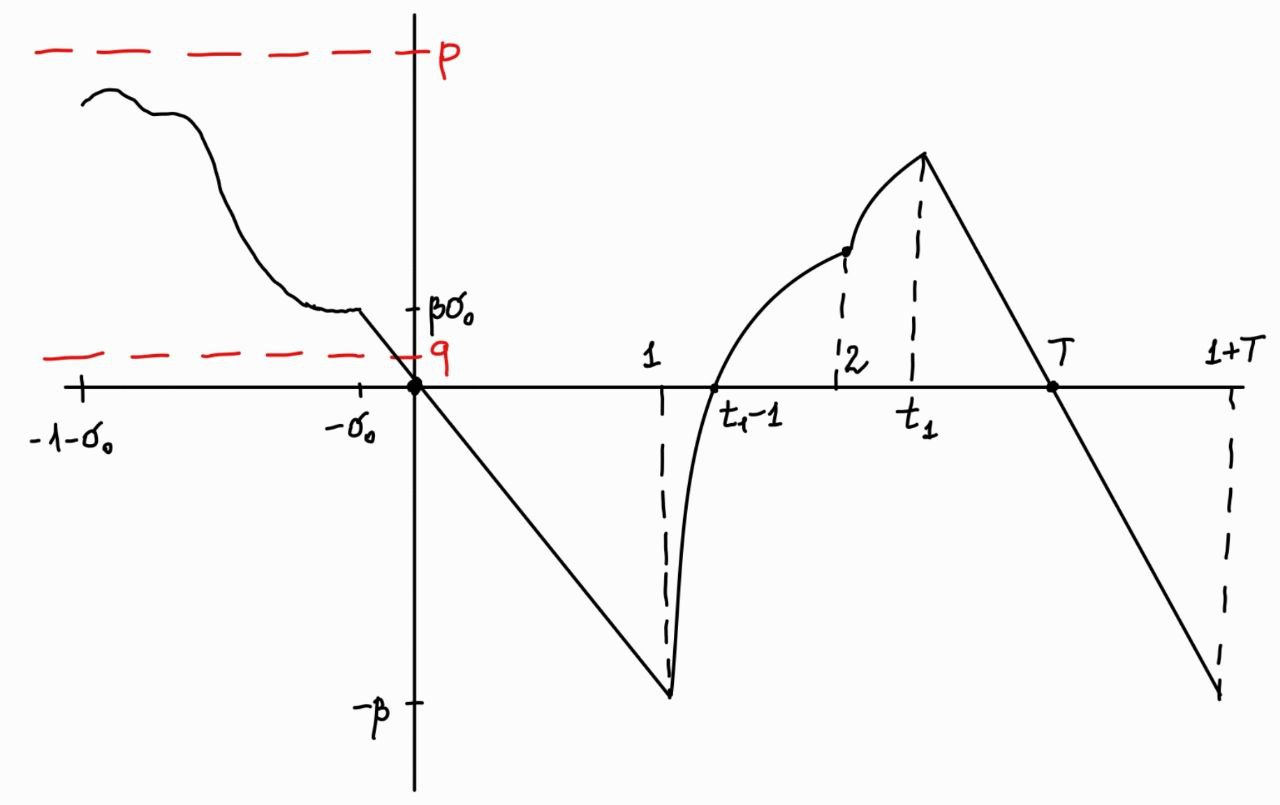
\includegraphics[width=0.8\linewidth]{func1.jpg}
    \end{center}
\end{frame}

\begin{frame}
	\frametitle{Основная теорема}
	\textbf{Теорема.} Пусть $S$ --- множество начальных функций,
	\[
	S = \{\varphi \in C[-1 - \sigma_0] \, | \, 0 < q \leq \varphi(t) \leq p, \, \varphi(-\sigma_0) = \beta \sigma_0\}.
	\]
	
	Тогда (при некоторых ограничениях на параметры $\alpha, \beta$) для произвольной $\varphi \in S$ и достаточно больших $\gamma$ уравнение \eqref{eq:MG_x} имеет решение $x^*_\gamma(t, \varphi)$ периода $T_{\gamma, \varphi}$, причём
	
	\[
	\lim\limits_{\gamma \to +\infty} \max\limits_{t \in [-\sigma_0, T_{\gamma, \varphi} + \sigma_0]} |x^*_\gamma(t, \varphi) - x^*(t)| = 0,
	\]
	
	\[
	\lim\limits_{\gamma \to +\infty} T_{\gamma, \varphi} = T
	\]
\end{frame}

\begin{frame}
	\frametitle{Вычисление асимптотики}
	Пусть
	$$\delta = \gamma^{-\nu}, \quad \nu \in (1/2, 1).$$
	%
	Вне окрестностей точек излома $t_0$ и $t_1$ ищем решение в виде
	\[
	x^*_\gamma(t, \varphi) = x^*(t) + \Delta(t, \varphi).
	\]
	
	При $t \in [t_i - \delta, t_i + \delta]$ ищем решение в виде
	\[
	x^*_\gamma(t, \varphi) = x^*(t_i) + \frac{1}{\gamma} w_i(\tau)|_{\tau = \gamma(t - t_i)} + \Delta(t, \varphi).
	\]
	%
    \[
    w_i(\tau) = -\beta \tau - \dfrac{\alpha e^{-x^*(t_i)}}{\dot{x}^*(t_i - 1)} \ln\left(e^{-\dot{x}^*(t_i - 1)\tau} + 1\right) \, \text{при} \, \dot{x}^*(t_i - 1) > 0,
    \]
    \[
    w_i(\tau) = (-\beta + \alpha e^{-x^*(t_i)})\tau - \dfrac{\alpha e^{-x^*(t_i)}}{\dot{x}^*(t_i - 1)} \ln\left(e^{\dot{x}^*(t_i - 1)\tau} + 1\right) \, \text{при} \, \dot{x}^*(t_i - 1) < 0,
    \]
\end{frame}

\begin{frame}
	\frametitle{Существование периодического решения}
	
	
\end{frame}

\section{Часть II. Дискретные бегущие волны в полносвязной цепи осцилляторов Мэки--Гласса}


\begin{frame}
	\frametitle{Полносвязная цепь осциляторов Мэки--Гласса}
	
	\begin{equation*}
		\label{eq:system_full_generators}
		\dfrac{d V_{j}}{dt}=- bV_{j} + \dfrac{ac\left(V_{j}(t - \tau) + \sum\limits_{k = 0, k\neq j}^{m}V_{k}(t)\right)}{1 + \left(c\left(V_{j}(t - \tau) + \sum\limits_{k = 0, k\neq j}^{m}V_{k}(t)\right)\right)^{\gamma}}, \quad j=0,1,\ldots,m.
	\end{equation*}
	
	$a, b, c, \tau > 0$, $\gamma \gg 0$
\end{frame}

\begin{frame}
	\frametitle{Полносвязная цепь осциляторов Мэки--Гласса}
	
	После перенормировок и предельного перехода при $\gamma \to +\infty$:
	
	\begin{equation*}
		\dot{u}_j=-\beta u_j+\alpha\left(u_j(t-1)+ \sum\limits_{k=0, k\neq j}^{m} u_{k}(t)\right)F\left(u_j(t-1)+\sum\limits_{k=0, k\neq j}^{m} u_{k}(t)\right).
	\end{equation*}

%	\begin{equation}
%		\label{eq:mg_relay_w}
%		\dot{u}=-\beta u+\alpha w(t) F(w(t)), \text{ где }
%	\end{equation}
%	%
%	\begin{equation*}
%	w(t) = \sum\limits_{s = 0}^m u(t - \tau_s).
%	\end{equation*}
\end{frame}


\begin{frame}
	\frametitle{Дискретная бегущая волна}
	
	\begin{equation}
		\label{eq:discrete_wave}
		u_j(t) = u(t + k_j\Delta),   
	\end{equation}
	где $\{k_0, k_1, \ldots, k_m\}$ --- перестановка номеров $\{0, 1, \ldots, m\}$, $u(t)$ --- некоторая $T-$периодическая функция, $\Delta > 0$ --- сдвиг.
	
	\small
	\begin{equation}
		\label{eq:mg_relay_0}
		\dot{u} = -\beta u+\alpha\left(u(t-1)+ \sum_{s=0,s\neq j}^{m}u(t+(k_s-k_j)\Delta)\right)F\left(\dots\right).
	\end{equation}
	\normalsize
	
	Если $u(t + (m + 1)\Delta) = u(t)$, т.е. 
	\[(m + 1)\Delta = pT \text{ для некоторого } p \in \mathbf{N},\]
	
	все уравнения системы обращаются в
	
	\small
	\begin{equation}
		\label{eq:mg_relay_0}
		\dot{u} = -\beta u+\alpha\left(u(t - 1) + \sum_{s=1}^{m}u(t + s\Delta)\right)F\left(\dots\right).
	\end{equation}
	\normalsize
	
	
\end{frame}

\begin{frame}
	\frametitle{Решение вспомогательного уравнения}
	\small
	\begin{equation*}
		\label{eq:u_star}
		u_*(t)=
		\begin{cases}
			u_0 e^{-\beta t}(\alpha A(t-t_0)+1) & \text{ при } t\in[t_0,t_0+1].
			\\
			u_0 e^{-\beta t}\left(\frac{\alpha^2}{2}Ae^{\beta}(t-t_0-1)^2+\alpha A(t-t_0)+1\right) & \text{ при } t\in[t_0+1,t_1],
			\\
			u_0 e^{-\beta t}\left(\frac{\alpha^2}{2}Ae^{\beta}(t_1-t_0-1)^2+\alpha A(t_1-t_0)+1\right) & \text{ при } t\in[t_1,t_0+T].
		\end{cases}
	\end{equation*}
	\normalsize
	%
	\[
	u_*(t+T)\equiv u_*(t),
	\]
	%
	\begin{equation*}
		\label{eq:mg_period_T}
		T = \dfrac{1}{\beta}\ln\left( \frac{\alpha^2}{2}Ae^{\beta}(t_1-t_0-1)^2+\alpha A(t_1-t_0)+1\right). 
	\end{equation*}
	
	Здесь $A = e + e^{\Delta} + e^{2\Delta} + \ldots + e^{m\Delta}$, $t_0$, $t_1$ --- точки переключения.
	
	\begin{center}
		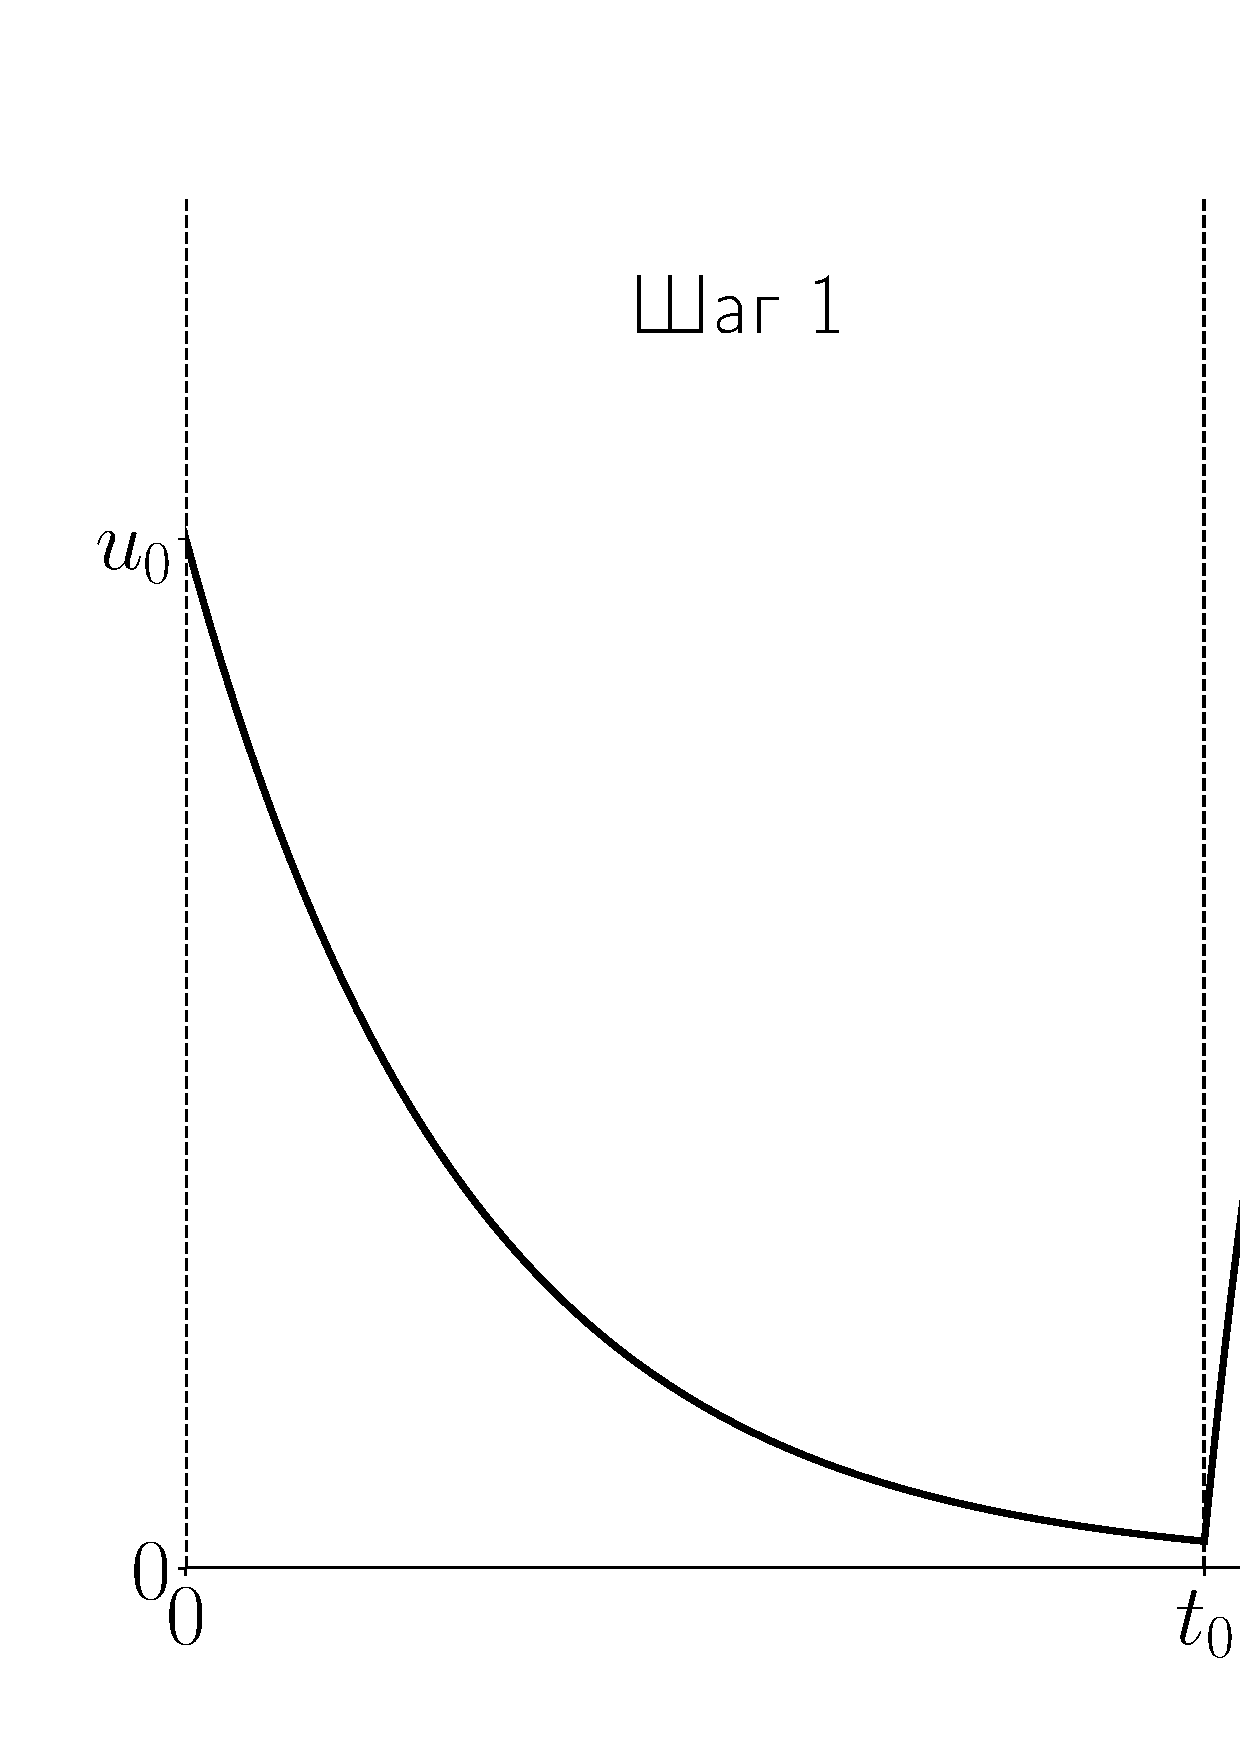
\includegraphics[width=0.6\textwidth]{u_star.png}
	
	\end{center}
\end{frame}

\begin{frame}
	\frametitle{Бегущая волна: теорема существования}
	
	\textbf{Теорема.} 
	Для произвольных $\beta > 0$, $\alpha \geqslant e^{\beta\left(1 + \frac{1}{e^{\beta}}\right)} - 1$ найдётся $\Delta > 1$, при котором вспомогательное уравнение с параметрами $\alpha, \beta, \Delta$ имеет $T$-периодическое решение, причём $T = (m + 1) \Delta$. Соответствующий набор функций $u_j(t) = u(t + j \Delta), j = 0, \ldots m$ (с точностью до нумерации компонент) является решением в виде дискретной бегущей волны.
\end{frame}

\begin{frame}
	\frametitle{Бегущая волна: численные результаты}
	
	\begin{center}
		\includegraphics[width=0.8\linewidth]{a5p0_b1p2_m2_solution_start.png}
		
		\includegraphics[width=0.8\linewidth]{a5p0_b1p2_m2_const_start.png}
		
		\includegraphics[width=0.8\linewidth]{a5p0_b1p2_m2_random_start.png}
	\end{center}
\end{frame}

\begin{frame}
	\frametitle{Двухластерная синхронизация в полносвязной системе}
	
\end{frame}

\begin{frame}
	\frametitle{Двухластерная синхронизация в полносвязной системе}
	
	\begin{equation}
		\label{eq:mg_cluster_system_norm}
		\begin{cases}
			\dot{u} = -\beta u + \alpha \, \Phi \big(u(t - 1) + \delta (m - 1) u + \delta n v\big),\\
			\dot{v} = -\beta v + \alpha  \, \Phi \big(v(t - 1) + \delta m u + \delta (n - 1) v\big).
		\end{cases},
	\end{equation}
	
	где 
	\begin{equation*}
		\Phi(x) = \dfrac{x}{1 + x^\gamma}.
	\end{equation*}
	
	После замен
	\begin{equation}
		\label{eq:tilde_change}
		\tilde{u}(t) = u(t - 1) + \delta (m - 1) u + \delta n v, \quad \tilde{v}(t) = v(t - 1) + \delta m u + \delta (n - 1) v,
	\end{equation}
	
	Получаем
	\begin{equation}
		\label{eq:mg_cluster_system_tilde}
		\begin{cases}
			\dot{\tilde{u}} = -\beta \tilde{u} + \alpha \big(\Phi(\tilde{u}(t - 1)) + \delta (m - 1) \, \Phi(\tilde{u}) + \delta n \, \Phi(\tilde{v})\big),\\
			\dot{\tilde{v}} = -\beta \tilde{v} + \alpha \big(\Phi(\tilde{v}(t - 1)) + \delta m \, \Phi(\tilde{u}) + \delta (n - 1) \, \Phi(\tilde{v})\big).
		\end{cases}
	\end{equation}
\end{frame}

\begin{frame}
	\frametitle{Двухластерная синхронизация в полносвязной системе}
	
	После экспоненциальной замены
	\begin{equation}
		\label{eq:exp_change}
		\tilde{u} = e^x, \quad \tilde{v} = e^y
	\end{equation}
	и ввода функцию $G(x) = e^{-x} \, \Phi (e^x)$, получаем итоговый вид системы:
	\begin{equation}
		\label{eq:system_main}
		\begin{cases}
			\dot{x} = -\beta + \alpha \left(e^{x(t - 1) - x} G(x(t - 1)) + \delta (m - 1) G(x) + \delta n e^{y - x} G(y)\right),\\
			\dot{y} = -\beta + \alpha \left(e^{y(t - 1) - y} G(y(t - 1)) + \delta m e^{x - y} G(x) + \delta (n - 1) G(y)\right).
		\end{cases}
	\end{equation}
\end{frame}

\section{Часть III. Режимы двухкастерной синхронизации в полносвязной цепи осцилляторов Мэки--Гласса}
\begin{frame}[allowframebreaks]
	\frametitle{Решение системы}
	\footnotesize
	\begin{equation*}
		\begin{cases}
			x = x_0 - \beta t,\\
			y = y_0 - \beta t
		\end{cases}
		\text{при } t \in [0, t_0], \text{ где } t_0 = \dfrac{y_0}{\beta};
	\end{equation*}
	%
	\begin{equation*}
		\begin{cases}
			x = x_0 - \beta t + \ln\left(1 + \frac{n}{n - 1} e^{-x_0 + \beta t_0}  (e^{\beta  (t - t_0)} - 1)\right),\\
			y = 0
		\end{cases}
		\text{при } t \in [t_0, t_0 + 1];
	\end{equation*}
	%
	\begin{multline*}
		\begin{cases}
			x = -\beta t + \ln\left(e^{x(t_{2i} + 1) + \beta (t_{2i} + 1)} + \frac{n (\delta(n - 1) - 1)}{\delta (n - 1)^2} (e^{\beta t} - e^{\beta (t_{2i} + 1)})\right)
			,\\
			y = 0.
		\end{cases}\\
		\text{при } t \in [t_{2i} + 1, t_{2i + 1}];
	\end{multline*}
	%
	\begin{multline*}
		\begin{cases}
			x = 0,\\
			y = -\beta t + \ln\left(e^{\beta t_{2i + 1}} + \left(\frac{1}{\delta(n - 1)} + \frac{m}{m - 1}\right) (e^{\beta t} - e^{\beta t_{2i + 1}})\right)
		\end{cases}\\
		\text{при } t \in [t_{2i + 1}, t_{2i} + 2];
	\end{multline*}
	%
	\begin{multline*}
		\begin{cases}
			x = 0,\\
			y = -\beta t + \ln\left(e^{y(t_{2i} + 2) + \beta (t_{2i} + 2)} + \left(\frac{\delta(n - 1) - 1}{\delta^2 (n - 1)^2} + \frac{m}{m - 1}\right) (e^{\beta t} - e^{\beta (t_{2i} + 2)})\right)
		\end{cases}\\
		\text{при } t \in [t_{2i} + 2, t_{2i + 1} + 1];
	\end{multline*}
	%
	\begin{multline*}
		\begin{cases}
			x = 0,\\
			y = -\beta t + \ln\left(e^{y(t_{2i + 1} + 1) + \beta(t_{2i + 1} + 1)} + \frac{m (\delta (m - 1) - 1)}{\delta (m - 1)^2} (e^{\beta t} - e^{\beta (t_{2i + 1} + 1)}) \right)
		\end{cases}\\
		\text{при } t \in [t_{2i + 1} + 1, t_{2i + 2}];
	\end{multline*}
	%
	\begin{multline*}
		\begin{cases}
			x = -\beta t + \ln\left(e^{\beta t_{2i + 2}} + \left(\frac{1}{\delta(m - 1)} + \frac{n}{n - 1}\right) (e^{\beta t} - e^{\beta t_{2i + 2}})\right),\\
			y = 0
		\end{cases}\\
		\text{при } t \in [t_{2i + 2}, t_{2i + 1} + 2];
	\end{multline*}
	%
	\begin{multline*}
		\begin{cases}
			x = -\beta t + \ln\left(e^{x(t_{2i + 1} + 2) + \beta (t_{2i + 1} + 2)} + \left(\frac{\delta(m - 1) - 1}{\delta^2 (m - 1)^2} + \frac{n}{n - 1}\right) (e^{\beta t} - e^{\beta (t_{2i + 1} + 2)})\right),\\
			y = 0
		\end{cases}\\
		\text{при } t \in [t_{2i + 1} + 2, t_{2i + 2} + 1];
	\end{multline*}
	%
	\begin{multline*}
		\begin{cases}
			x = -\beta t + \ln\left(e^{y(t_{2i + 2} + 1) + \beta(t_{2i + 2} + 1)} + \frac{n (\delta(n - 1) - 1)}{\delta (n - 1)^2} (e^{\beta t} - e^{\beta (t_{2i + 2} + 1)}) \right),\\
			y = 0
		\end{cases}\\
		\text{при } t \in [t_{2i + 2} + 1, t_{2i + 3}].
	\end{multline*}
	\normalsize
\end{frame}

\begin{frame}
	\frametitle{Решение системы}
	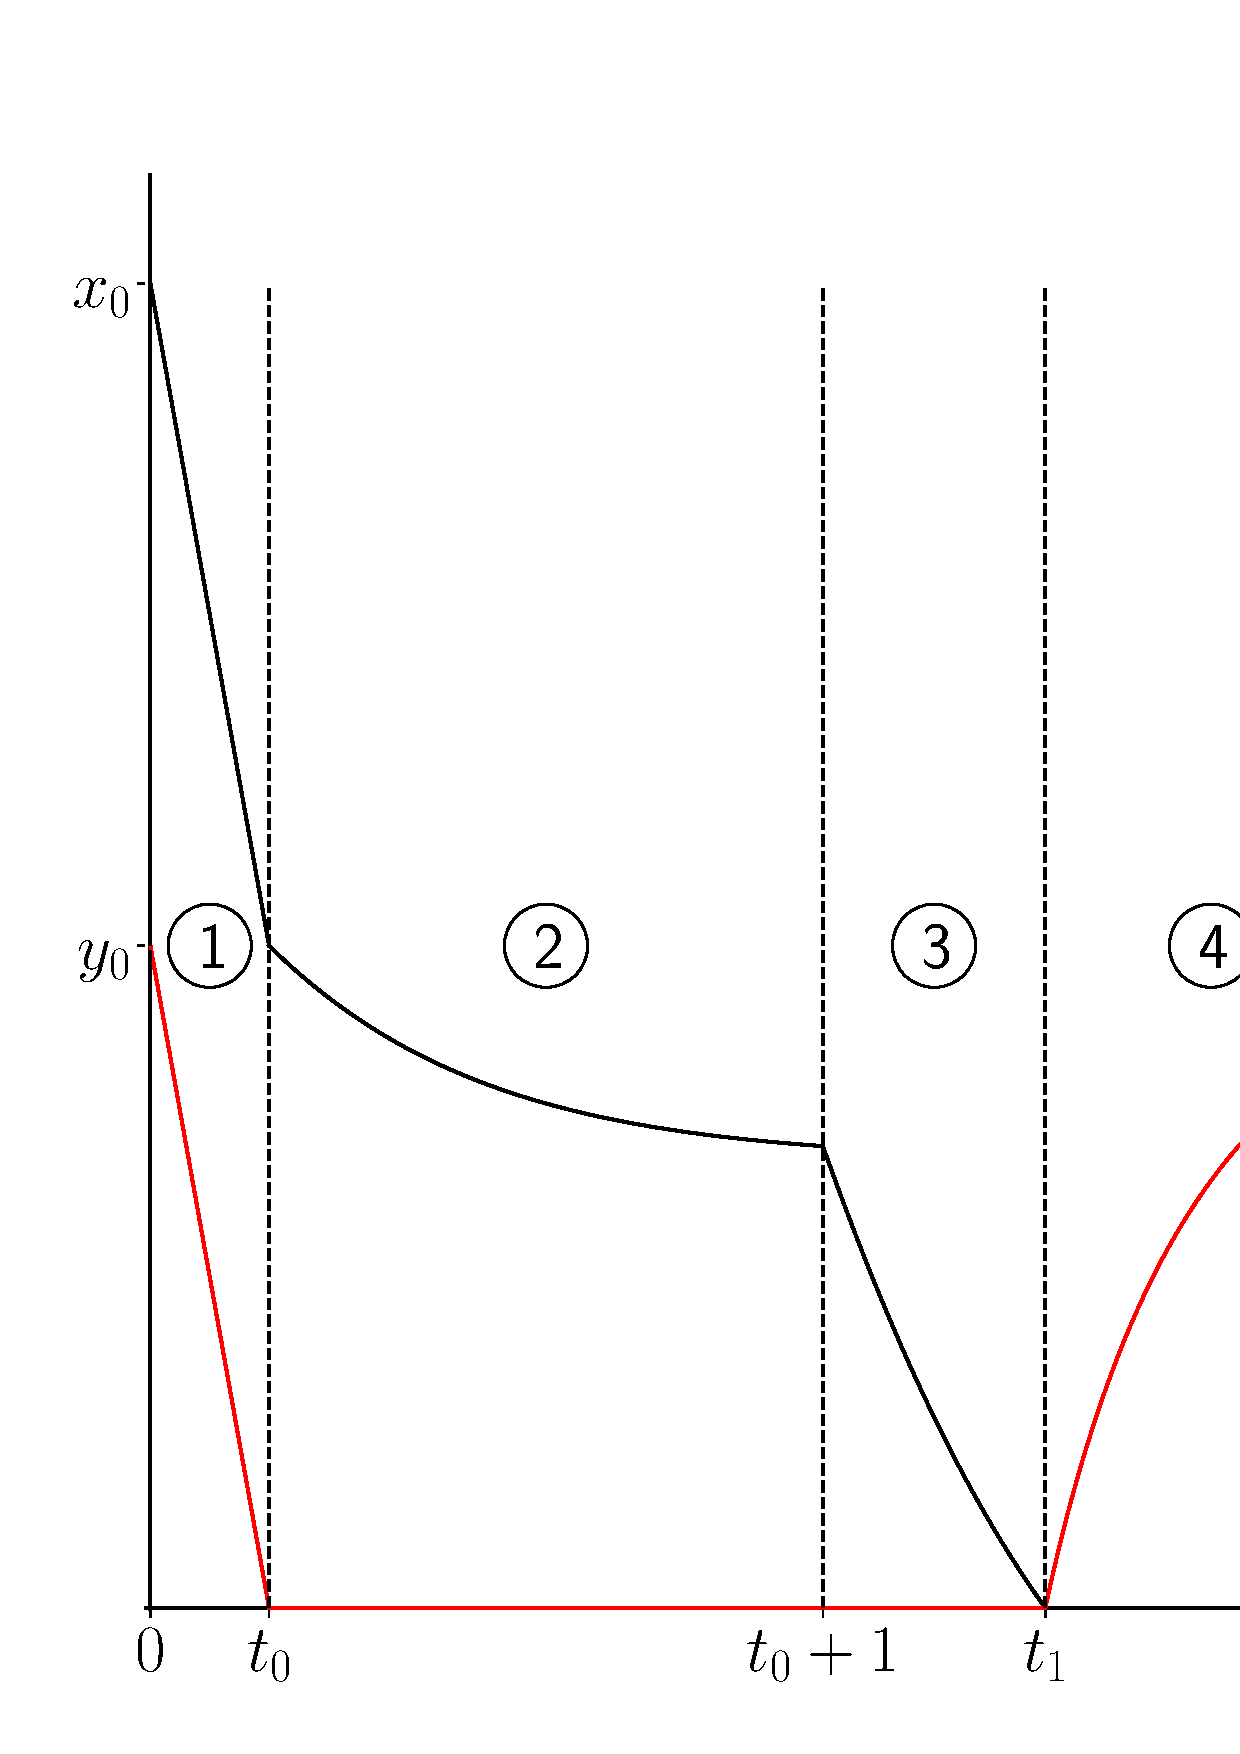
\includegraphics[width=\linewidth]{cluster_step_by_step.png}
\end{frame}


\begin{frame}
	\frametitle{Теорема существования}
	\textbf{Теорема.} При ограничениях на параметры 
	\small
	\begin{equation*}
		\label{eq:constraint_2}
		\beta < \alpha \delta (m - 1), \quad \beta < \alpha \delta (n - 1),
	\end{equation*}
	\begin{equation*}
		\label{eq:constraint_3}
		e^{\beta} \cdot \dfrac{n - \delta(n - 1)}{\delta (n - 1)^2} > \dfrac{1}{n - 1} + \dfrac{1}{\delta(m - 1)}, \quad
		e^{\beta} \cdot \dfrac{m - \delta(m - 1)}{\delta (m - 1)^2} > \dfrac{1}{\delta(n - 1)} + \dfrac{1}{m - 1}.
	\end{equation*}
	\normalsize
	существует периодическое решение $x(t)$, $y(t)$, соответствующее шагам 4--9 решения, описанного выше.
	
\end{frame}


\begin{frame}
	\frametitle{Численные результаты}
	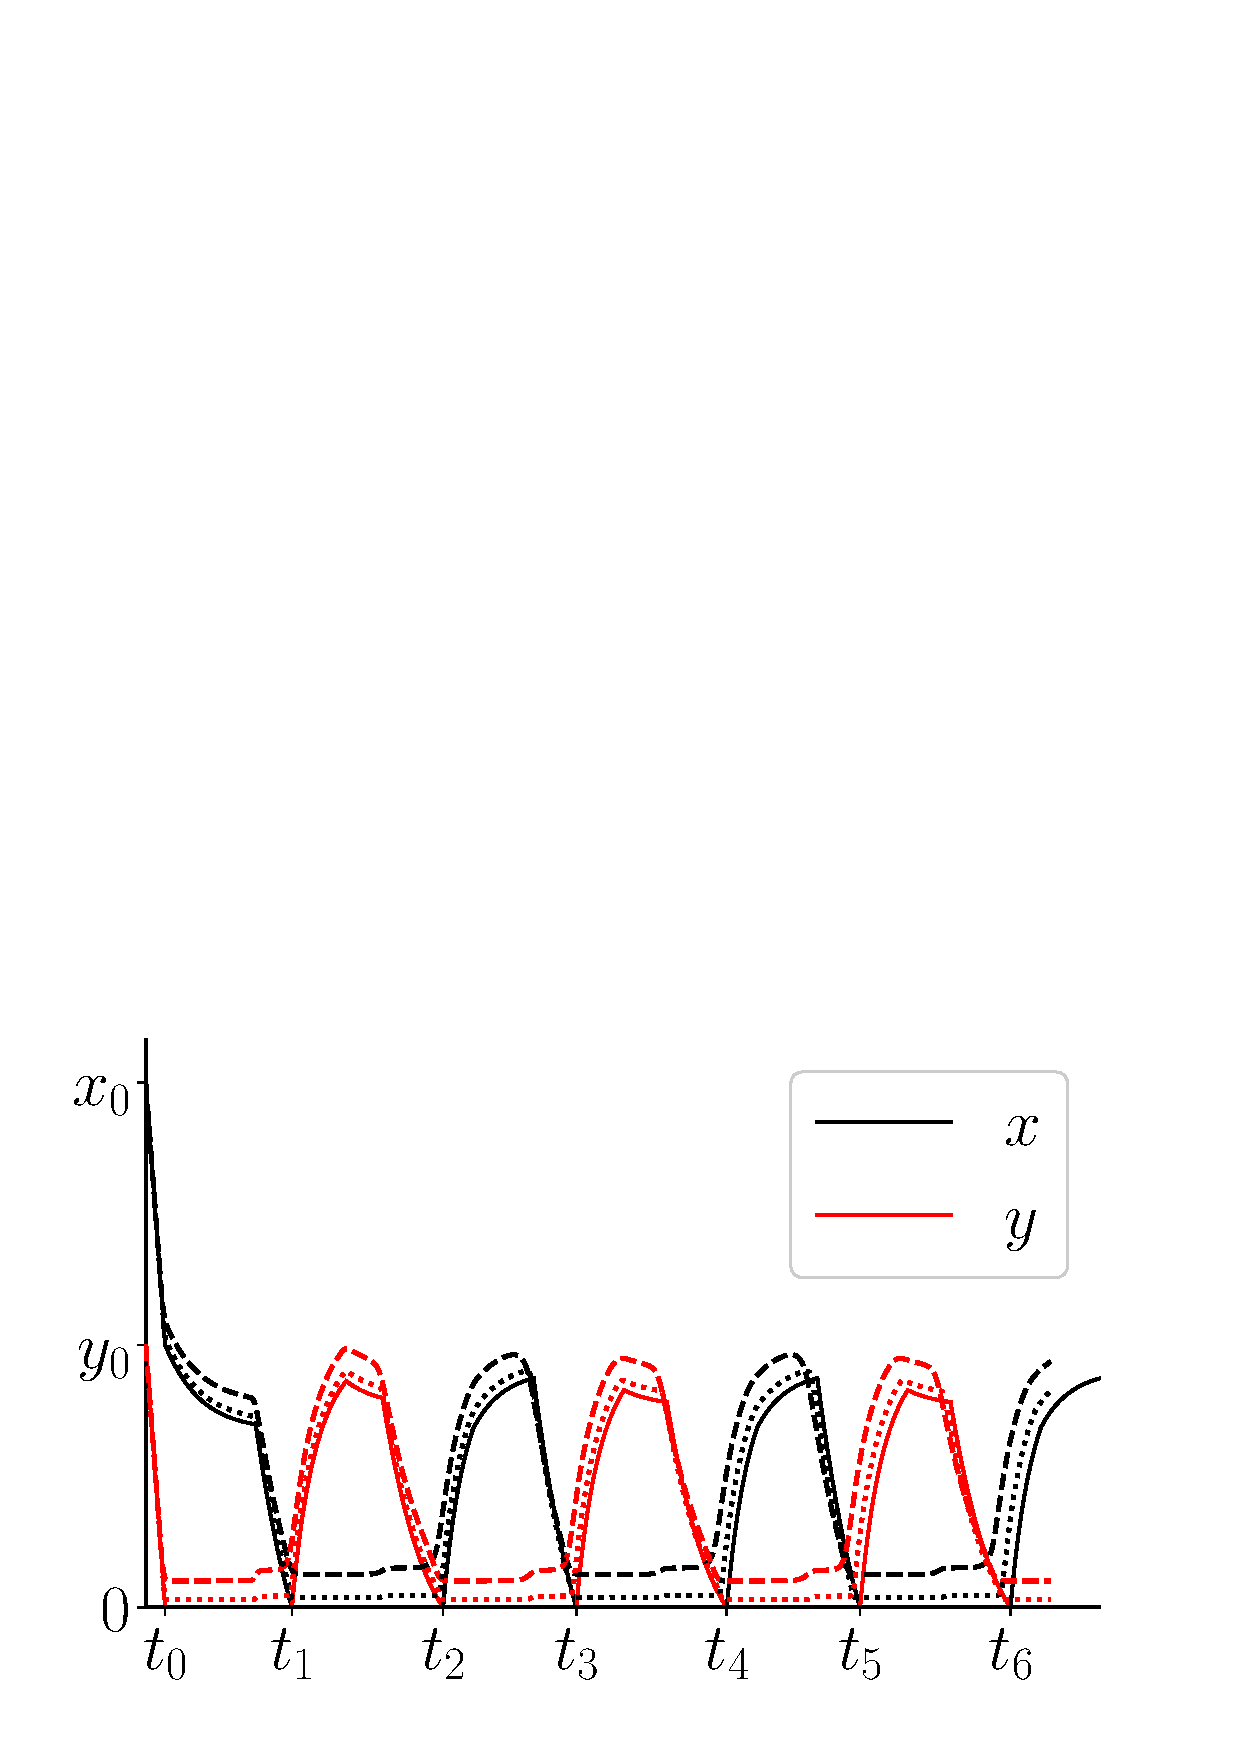
\includegraphics[width=0.66\linewidth]{cluster_solution.png}
	\hfill
	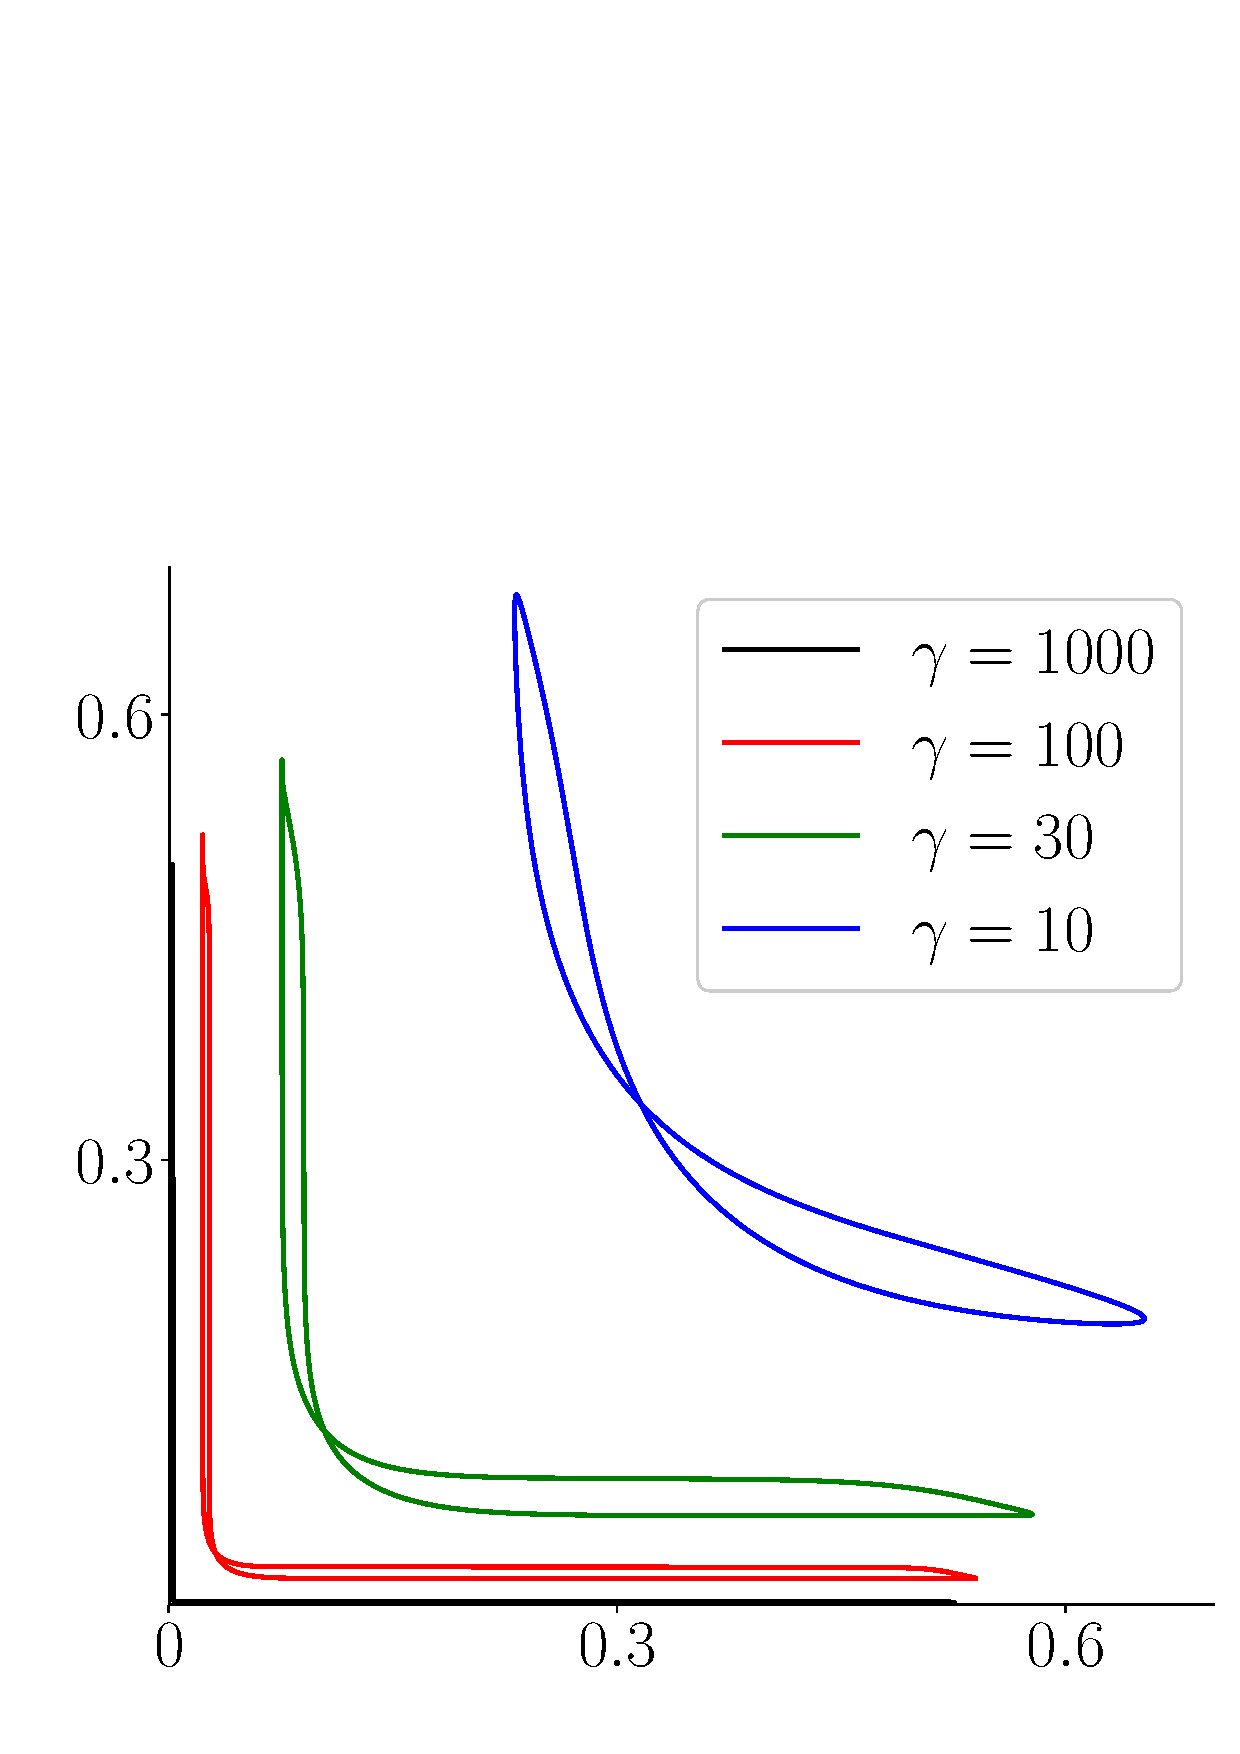
\includegraphics[width=0.33\linewidth]{cluster_phase_portrait.png}
\end{frame}
       % Настройки заглавной странице
\begin{frame}
    \frametitle{Научная новизна}
    \begin{itemize}
    	\item Впервые получены асимптотические формулы решения уравнения Мэки--Гласса по параметру $\gamma^{-\nu} \ll 1$ и доказано существование периодических решений при ограничении на параметры $\alpha > \exp\left(\beta(1 + e^{-\beta})\right)$.
    	\item Впервые доказано существование периодических режимов в виде дискретной бегущей волны в полносвязной сети релейных генераторов Мэки--Гласса, а также сформулированы и доказаны условия их существования в виде ограничения на параметры соответствующей системы дифференциальных уравнений с запаздыванием.
    	\item Впервые доказано существование периодических режимов двухкластерной синхронизации в полносвязной сети релейных генераторов Мэки--Гласса, а также сформулированы и доказаны условия их существования в виде ограничения на параметры соответствующей системы дифференциальных уравнений с запаздыванием.
    \end{itemize}
\end{frame}
\note{
    Проговаривается вслух научная новизна
}

\begin{frame} % публикации на одной странице
	\frametitle{Список публикаций}
	\begin{itemize}
		\item[{[1]}] Two-cluster synchronization on a fully coupled network of Mackey--Glass generators // V.~Alekseev // Partial Differential Equations in Applied Mathematics. --- 2024. --- Vol. 12. --- P. 100930.
		\item[{[2]}] Existence of Discrete Traveling Waves in Fully Coupled Network of Mackey--Glass Relay Generators / V.~Alekseev, M.~Preobrazhenskaia, V.~Vorontsova // Differential Equations. --- 2024. --- Vol. 60, No 9.
		\item[{[3]}] Анализ асимптотической сходимости периодического решения уравнения Мэки--Гласса к решению предельного релейного уравнения / В.~В.~Алексеев, М.~М.~Преображенская // Теоретическая и математическая физика. --- 2024. --- Т. 220, № 2. --- С. 213--236.
		\item[{[4]}] Сергеев, И.Н. О семинаре по качественной теории дифференциальных уравнений в московском государственном университете имени М.В. Ломоносова // Дифференциальные уравнения. --- 2024. --- Т. 60, № 11. --- С. 1566--1584.
    \end{itemize}
\end{frame}
\note{
    Результаты работы опубликованы в N печатных изданиях,
    в~т.\:ч. M реферируемых изданиях.
}

\begin{frame}
    \frametitle{Выступления на семинарах}
    \begin{itemize}
    	\item Семинар кафедры <<Функциональный анализ и его приложения>> Владимирского государственного университета, 13~февраля~2025~года.
        \item Семинар по качественной теории дифференциальных уравнений в московском государственном университете имени М.В.~Ломоносова, 29~ноября~2024 года.\\\texttt{https://www.elibrary.ru/item.asp?id=75144298}
        \item Научный семинар лаборатории динамических систем и приложений НИУ ВШЭ в Нижнем Новгороде, 25~сентября~2024~года.\\\texttt{https://nnov.hse.ru/bipm/dsa/semtmd}.
        \item Семинар по нелинейной динамике Ярославского государственного университета, 19~сентября~2024~года.\\\texttt{https://cis.uniyar.ac.ru/index.php/event/460}.
    \end{itemize}
\end{frame}
\note{
    Работа была представлена на ряде конференций.
}

\begin{frame}
	\frametitle{Участие в конференциях}
	\begin{itemize}
		\item Конференция <<Integrable Systems and Nonlinear Dynamics>> (ISND – 2024), Ярославль,~2024.
		\item Конференция <<Topological Methods in Dynamics and Related Topics VII>>, Нижний Новгород,~2024.
		\item Международная конференция по дифференциальным уравнениям и динамическим системам DIFF-2024, Суздаль,~2024.
		\item Конференция <<Нелинейные дни в Саратове для молодых>>, Саратов, 2023.
		\item Конференция <<Satellite International Conference on Nonlinear Dynamics {\&} Integrability>>, Ярославль,~2022.
		\item Международная конференция по дифференциальным уравнениям и динамическим системам DIFF--2022, Суздаль,~2022.
	\end{itemize}
\end{frame}
\note{
	Работа была представлена на ряде конференций.
}

\begin{frame}[plain, noframenumbering] % последний слайд без оформления
    \begin{center}
        \Huge
        Спасибо за внимание!
    \end{center}
\end{frame}
    % Последние слайды презентации
%\appendix
%\chapter{Примеры вставки листингов программного кода}\label{app:A}

      % Запасные слайды презентации
\end{document}
